% -*- coding: utf-8 -*-
% =============================================================================
% 北京邮电大学研究生学位论文 LaTeX 模板工程 (符合 GB/T 7713.1-2006 规范)
% 专业领域：电子信息（专业代码：085402 通信工程）
% 研究方向：面向低空智联网的无人机通感一体化波形设计与感知辅助通信资源管理
% TODO: 待对照北邮官方模板校准封面格式与校徽布局
% =============================================================================

\documentclass[12pt,a4paper,openany,UTF8]{ctexrep}

% -----------------------------------------------------------------------------
% 页面尺寸与版面几何布局 (BUPT Thesis Layout)
% -----------------------------------------------------------------------------
\usepackage{geometry}
\geometry{
  top=3.0cm,
  bottom=2.5cm,
  left=2.6cm,
  right=2.6cm,
  headheight=15pt,
  headsep=18pt,
  footskip=25pt
}

% -----------------------------------------------------------------------------
% 数学公式与符号支持
% -----------------------------------------------------------------------------
\usepackage{amsmath,amssymb,amsfonts,amsthm,bm}
\newtheorem{theorem}{定理}[chapter]
\newtheorem{lemma}{引理}[chapter]
\newtheorem{definition}{定义}[chapter]

% -----------------------------------------------------------------------------
% 图表、三线表与算法环境支持 (GB/T 7713 规范禁用双竖线，强制 booktabs)
% -----------------------------------------------------------------------------
\usepackage{booktabs}
\usepackage{tabularx}
\usepackage{array}
\usepackage{graphicx}
\usepackage{caption}
\usepackage{subcaption}
\captionsetup{font={small},labelfont={bf},skip=6pt}

\usepackage{algorithm}
\usepackage{algorithmic}

% 页眉页脚排版
\usepackage{fancyhdr}
\pagestyle{fancy}
\fancyhf{}
\fancyhead[C]{\small 北京邮电大学硕士学位论文：\leftmark}
\fancyfoot[C]{\small \thepage}
\renewcommand{\headrulewidth}{0.75pt}
\renewcommand{\footrulewidth}{0pt}

% -----------------------------------------------------------------------------
% 超链接与受控 TODO 占位符
% -----------------------------------------------------------------------------
\usepackage{xcolor}
\providecommand{\TODO}[1]{\textcolor{red}{\textbf{[TODO: #1]}}}

\usepackage{hyperref}
\hypersetup{
  colorlinks=true,
  linkcolor=black,
  citecolor=black,
  urlcolor=black,
  pdfauthor={北京邮电大学硕士研究生},
  pdftitle={面向低空智联网的无人机通感一体化波形设计与感知辅助通信资源管理}
}
\pdfstringdefDisableCommands{\def\bm#1{#1}}

% -----------------------------------------------------------------------------
% 正文开始
% -----------------------------------------------------------------------------
\begin{document}

% 论文封面 (Title Page)
\begin{titlepage}
  \centering
  \vspace*{1.2cm}
  {\Huge \textbf{北\quad 京\quad 邮\quad 电\quad 大\quad 学}\par}
  \vspace{0.5cm}
  {\Large \textbf{BEIJING UNIVERSITY OF POSTS AND TELECOMMUNICATIONS}\par}
  \vspace{1.2cm}
  {\Large \textbf{硕\quad 士\quad 学\quad 位\quad 论\quad 文}\par}
  \vspace{1.5cm}
  {\LARGE \textbf{面向低空智联网的无人机通感一体化波形设计}\par}
  \vspace{0.3cm}
  {\LARGE \textbf{与感知辅助通信资源管理研究}\par}
  \vspace{0.8cm}
  {\large \textit{Waveform Design and Sensing-Assisted Communication Resource}\par}
  {\large \textit{Management for UAV-Enabled ISAC in Low-Altitude Internet of Things}\par}
  \vfill
  \begin{tabular}{ll}
    \textbf{姓\qquad 名}： & 硕士研究生 \\
    \textbf{学\qquad 号}： & 2408540201 \\
    \textbf{学\qquad 院}： & 信息与通信工程学院 \\
    \textbf{专业领域}：   & 电子信息（专业代码：085402 通信工程） \\
    \textbf{研究方向}：   & 低空移动通信与通感融合信号处理 \\
    \textbf{指导教师}：   & 教授 \\
  \end{tabular}
  \vspace{1.2cm}
  \par
  {\large \textbf{二〇二六年九月}\par}
\end{titlepage}

% 中英文摘要与目录 (前言采用罗马数字页码)
\pagenumbering{Roman}
\setcounter{page}{1}

% 原创性声明与使用授权说明
\chapter*{北京邮电大学学位论文原创性声明与使用授权说明}
\thispagestyle{empty}
\noindent 本人郑重声明：所呈交的学位论文，是本人在导师的指导下，独立进行研究工作所取得的成果。除文中已经注明引用的内容外，本论文不含任何其他个人或集体已经发表或撰写过的作品成果。对本文的研究做出重要贡献的个人和集体，均已在文中以明确方式标明。本人完全意识到本声明的法律结果由本人承担。

\vspace{1.5cm}
\begin{flushright}
  学位论文作者签名：\underline{\hspace{3cm}} \qquad
  签字日期：\qquad 年\quad 月\quad 日
\end{flushright}
\newpage

% 中文摘要
\chapter*{摘\quad 要}
\addcontentsline{toc}{chapter}{摘要}

随着低空经济上升为国家战略性新兴产业，低空智联网（LA-IoT）作为保障海量低空飞行器安全巡航、协同调度与数据交互的关键数字化基础设施，其网络感知与通信能力面临着前所未有的严苛挑战。低空空域飞行器具有低空、慢速、小雷达截面等特征，加之复杂低空环境下的严重建筑物物理遮挡与高动态空地多普勒扩展，传统分立的通信基站与雷达站架构面临部署成本高昂、空域盲区广泛以及频谱冲突加剧的现实瓶颈。

通感一体化（ISAC）技术通过频谱共享、硬件复用与基带联合信号处理，为低空智联网构建了全域感知与高效传输深度融合的新途径。针对低空空域中感知精度与通信速率相互挤占、加权和目标函数缺乏物理可解释性、以及资源分配组合规模爆炸三个核心困难，本文围绕低空无人机通感一体化系统的波束成形、子载波分配与功率控制展开研究，主要成果包括：
\begin{enumerate}
  \item \textbf{建立空地多载波通感一体化系统模型并推导角度估计 CRB 闭式解}：给出含收发阵列增益的雷达回波模型与导向矢量导数，推导出角度估计克拉美罗下界（CRB）的闭式表达式。指出文献中常见的 $N_{\mathrm{R}}^{-3}$ 标度源于信噪比按单阵元定义，而在回波幅度已吸收全部阵列增益的建模下正确标度为 $N_{\mathrm{R}}^{-2}$，并以蒙特卡洛仿真独立验证该结论（五组比值落在 $[0.951,\,1.050]$，最大偏差 5.0\%）。
  \item \textbf{论证加权和目标函数的物理不可解释性并建立等速率约束评价框架}：证明加权和形式在权重趋于零时退化为单一功能优化、且感知侧 CRB 出现发散的非物理奇点，因而其扫描曲线不能作为通感权衡的可靠依据。据此改用「在给定通信和速率约束下最小化 CRB」的等速率约束框架，使不同方案的比较具有明确前提。
  \item \textbf{提出迫零预编码与匹配感知波束联合的闭式功率分配构造，并证明感知子载波选择的最优性}：在给定感知波束的前提下，将功率分配化为一维单调问题并给出闭式解与临界感知功率表达式；对子载波选择问题，通过交换论证证明按单位功率通信效率升序选取的贪心策略最优，将指数规模的组合搜索降为一次排序，复杂度由 $O\bigl(\binom{M}{N_{\mathrm{s}}}\bigr)$ 降至 $O(M\log M)$。
  \item \textbf{设计交替 MMSE 波束与功率投影梯度上升的收敛算法，并完成全链路可复现仿真}：以零和投影方向结合 Armijo 回溯保证总功率守恒与目标单调上升，实测 8 次迭代内和速率由 9.6248 增至 9.7130~bps/Hz；轨迹层采用 SLSQP 求解，逐时隙 CRB 较匀速盘旋基线在第 30 时隙优 52.6 倍。全部仿真脚本、参数与原始数据随文提供，可逐行复算。
\end{enumerate}

\vspace{0.6cm}
\noindent \textbf{关键词}：低空智联网；无人机通信；通感一体化 (ISAC)；克拉美罗界 (CRB)；子载波分配；交替优化
\newpage

% 英文摘要
\chapter*{ABSTRACT}
\addcontentsline{toc}{chapter}{ABSTRACT}

Driven by the strategic expansion of the low-altitude economy, the Low-Altitude Internet of Things (LA-IoT) serves as an essential digital foundation to guarantee safe airspace operation, autonomous coordination, and reliable high-rate data transmission for massive unmanned aerial vehicles (UAVs). However, low-altitude aircraft typically exhibit low-altitude, slow-speed, and small-size (LSS) physical characteristics. Compounded by severe electromagnetic blockage in urban canyons and substantial Doppler shifts induced by high mobility, conventional disjoint communication and radar infrastructures suffer from prohibitive deployment costs, extensive sensing blind zones, and severe spectrum scarcity.

Integrated Sensing and Communication (ISAC) provides a viable path to deep integration of ubiquitous sensing and high-rate transmission for the Low-Altitude Internet of Things (LA-IoT) by sharing spectrum, hardware, and baseband processing. This thesis addresses three core difficulties in low-altitude UAV ISAC systems: the mutual encroachment between sensing accuracy and communication throughput, the lack of physical interpretability of weighted-sum objectives, and the combinatorial explosion of resource allocation. The main contributions are summarized as follows:
\begin{enumerate}
  \item \textbf{System modeling and closed-form CRB for angle estimation}: We establish a multicarrier ISAC model incorporating transmit/receive array gains in the radar echo, and derive a closed-form Cram\'er-Rao Bound (CRB) for angle estimation. We show that the $N_{\mathrm{R}}^{-3}$ scaling frequently quoted in the literature stems from a per-element signal-to-noise ratio definition; when the echo amplitude absorbs the full array gain, the correct scaling is $N_{\mathrm{R}}^{-2}$. This is independently verified by Monte-Carlo simulation, where the five ratios fall within $[0.951,\,1.050]$ with a maximum deviation of 5.0\%.
  \item \textbf{Physical critique of weighted-sum objectives and an equal-rate evaluation framework}: We prove that a weighted sum degenerates into single-function optimization as the weight vanishes, and that the sensing-side CRB exhibits a non-physical singularity. Its swept curve therefore cannot serve as a reliable basis for the sensing--communication trade-off. We instead adopt an equal-rate-constrained framework that minimizes the CRB subject to a prescribed communication sum rate, so that comparisons between schemes carry an explicit premise.
  \item \textbf{Closed-form power allocation with zero-forcing precoding and a matched sensing beam, and optimality of subcarrier selection}: Given the sensing beam, the power allocation reduces to a one-dimensional monotone problem with a closed-form solution and an explicit critical sensing power. For subcarrier selection, an exchange argument proves that the greedy rule, which selects subcarriers in ascending order of per-unit-power communication efficiency, is optimal. This reduces the combinatorial search from $O\bigl(\binom{M}{N_{\mathrm{s}}}\bigr)$ to a single sort of complexity $O(M\log M)$.
  \item \textbf{Convergent alternating MMSE beamforming with projected power gradient ascent, and a fully reproducible simulation}: A zero-sum projected direction combined with Armijo backtracking preserves the total power budget while guaranteeing monotone improvement of the objective; the sum rate rises from 9.6248 to 9.7130~bps/Hz within eight iterations. The trajectory layer is solved by SLSQP, and the per-slot CRB at the 30th slot is 52.6 times better than that of a constant-speed circular baseline. All simulation scripts, parameters, and raw data are provided so that every reported figure can be recomputed independently.
\end{enumerate}

\vspace{0.6cm}
\noindent \textbf{Keywords}: Low-Altitude Internet of Things; UAV Communications; Integrated Sensing and Communication (ISAC); Waveform Design; Cramér-Rao Bound (CRB); Alternating Optimization
\newpage

% 目录
\tableofcontents
\newpage

% 图目录与表目录
\listoffigures
\newpage
\listoftables
\newpage

% 主要符号对照表
\chapter*{主要符号对照表}
\addcontentsline{toc}{chapter}{主要符号对照表}
\begin{center}
\begin{tabular}{ll}
  \toprule
  \textbf{符号} & \textbf{含义说明} \\
  \midrule
  $\mathbf{X}$ & 发射通感一体化预编码基带波形矩阵 \\
  $\mathbf{H}_c$ & 通信下行多输入多输出（MIMO）等效信道矩阵 \\
  $\mathbf{H}_s$ & 感知目标回波散射空间信道矩阵 \\
  $\mathrm{CRB}$ & 目标运动与位置参数估计的克拉美罗界矩阵 \\
  $\mathbf{J}$ & 费雪信息矩阵（Fisher Information Matrix, FIM） \\
  $\mathrm{SINR}_k$ & 第 $k$ 个通信用户的接收信干噪比 \\
  $\sigma_c^2$ & 通信接收机加性复高斯白噪声方差 \\
  $\sigma_s^2$ & 感知接收机加性复高斯白噪声方差 \\
  $\mathbf{q}_u$ & 第 $u$ 架无人机的三维空间位置坐标向量 \\
  $V_{\max}$ & 无人机最大水平巡航线速度 \\
  $P_{\max}$ & 系统发射总功率预算 \\
  $\Delta f$ & OFDM 子载波间隔 \\
  $M$ & OFDM 正交子载波总数 \\
  $N_t$ & 基站/无人机发射天线数 \\
  $N_r$ & 感知接收天线数 \\
  $K$ & 通信移动用户总数 \\
  $U$ & 协同无人机总数 \\
  $\mathbf{W}$ & 下行多用户通信预编码矩阵 \\
  $\mathbf{w}_s$ & 感知定向探测波束赋形向量 \\
  $\alpha_k$ & 目标雷达散射截面积（RCS）及复反射系数 \\
  $\theta_k$ & 目标相对于天线阵列的到达角（AoA） \\
  $\tau_k$ & 目标信号往返传播时延 \\
  $f_{D,k}$ & 目标运动引起的多普勒频移 \\
  $R_{\mathrm{sum}}$ & 通信下行加权和速率 \\
  $\Gamma_{\mathrm{th}}$ & 通信接收最低 SINR 门限要求 \\
  \bottomrule
\end{tabular}
\end{center}
\newpage

% 正文部分 (阿拉伯数字页码)
\pagenumbering{arabic}
\setcounter{page}{1}

% -*- coding: utf-8 -*-
\chapter{绪论}
\label{chap:intro}

\section{研究背景与低空智联网业务演进}
\label{sec:background}

\subsection{低空经济与低空智联网的国家战略定位}
随着低空空域管理改革的纵深推进与通用航空技术的跨越式发展，以无人机（Unmanned Aerial Vehicle, UAV）为核心主体的低空经济已上升为国家战略性新兴产业。低空智联网（Low-Altitude Internet of Things, LA-IoT）作为支撑低空飞行器规模化运行的关键数字化基础设施，承担着空域安全监管、飞行器协同组网、超视距控制指令下达以及宽带载荷数据回传等多重任务。

从产业形态看，低空经济并非单一行业，而是由低空制造、低空飞行、低空保障与综合服务四个板块构成的复合生态。其典型应用场景包括城市末端物流配送、电力与油气长输管线巡检、农林植保作业、应急救援与医疗物资投送、城市空中交通（Urban Air Mobility, UAM）以及低空文旅观光等。这些场景对低空智联网提出的需求并不一致：物流配送要求高可靠的指令链路与精确的航路保持；管线巡检要求对沿线设施的高分辨率成像与缺陷识别；应急救援要求在有遮挡、强干扰的复杂地形下维持通信不中断；城市空中交通则要求对高密度飞行器流进行实时冲突探测与解脱。

需求的多样性直接决定了低空智联网不能沿用单一功能的传统架构。若按功能分别建设通信网、监视网与导航网，则在同一片空域内将出现多套射频前端、多组天线阵列与多份频谱占用，站址资源与能耗开销成倍增长，而频谱在低频段已高度紧张。这一矛盾在低空场景中尤为突出：低空飞行器数量大、密度高、更新快，若每一种新业务都需要新建一套专用基础设施，则基础设施建设速度将永远滞后于业务增长。

\subsection{低空监视的现实困境}
在低空空域（飞行高度通常在 1000 米以下）环境下，飞行环境呈现出三维立体、障碍密集与动态异构的特征。低空飞行器种类繁多，涵盖消费级航拍无人机、行业巡检多旋翼平台以及垂直起降电动飞行器（eVTOL）。这些目标普遍具有低空飞行、慢速巡航及雷达散射截面积较小的“低慢小”（Low-altitude, Slow-speed, Small-size, LSS）物理属性。

“低慢小”属性给传统监视手段带来了三重困难。其一是探测距离受限：雷达散射截面积小意味着回波功率微弱，在四次方衰减规律下，可探测距离被显著压缩。其二是杂波抑制困难：低空目标的多普勒频率与地物、植被、建筑物的杂波谱高度重叠，传统动目标显示（Moving Target Indication, MTI）滤波器难以在不损失目标能量的前提下剔除杂波。其三是遮挡与多径：城市低空环境中建筑物密集，地面雷达视线被频繁遮挡，形成大量探测盲区，而多径反射又会产生虚假点迹。

传统的地面二次雷达监视网络受限于地面建筑物理遮挡，存在严重的探测盲区与多径地杂波干扰；而若单独建设高密度专用雷达基站，将面临高昂的站址资源成本与频谱匮乏约束。这两条路径各自的困境，构成了本文研究的现实起点。

\subsection{通感一体化带来的技术契机}
在此背景下，通感一体化（Integrated Sensing and Communication, ISAC）技术应运而生。ISAC 旨在打破通信与雷达探测各自独立的传统烟囱式系统架构，通过在发射端共享射频前端硬件、天线阵列与无线频谱资源，利用联合设计的基带信号同时实现对空域目标的高精度环境感知与高速可靠无线通信传输。

将 ISAC 技术深度融合至低空无人机系统，可带来三个层面的收益。在基础设施层面，ISAC 能够复用现有移动通信蜂窝网络的广域覆盖优势，无需为感知功能单独选址建站，大幅降低部署成本与能耗开销。在频谱层面，ISAC 在同一段频谱上同时承载通信与感知，频谱效率相对于功能分离方案近似翻倍，这对低频段频谱已高度紧张的现实具有直接价值。在系统能力层面，感知获得的空域目标位置与运动状态可反哺通信的动态波束对准与链路资源调度，而通信网络的高密度基站又可提供多点协同的感知视角，二者形成正向增强而非简单叠加。

正是这一“一加一大于二”的潜力，使得 ISAC 被视为构建具备全域感知与自适应通信能力的低空泛在立体智联网络的核心使能技术。然而，潜力的兑现并非无条件：通信与感知在波形、功率、波束与子载波上的资源竞争是客观存在的物理事实，如何在资源受限前提下定量刻画并优化这一权衡，是本文要回答的核心问题。

\section{无人机通感一体化核心挑战与理论矛盾}
\label{sec:challenge}

将通感一体化技术引入高动态低空无人机场景，面临诸多基础理论挑战与工程实现矛盾：

\begin{enumerate}
  \item \textbf{波形多维时频空域资源博弈矛盾}：雷达探测需要恒模、低峰均功率比（PAPR）且具备理想二维模糊函数的探测波形以保障远距离探测灵敏度；而多载波宽带数字通信追求高阶正交幅度调制（QAM）以最大化频谱效率与香农信道容量。两者在多载波子载波功率分配与相位调制上存在天然的物理竞争关系。低 PAPR 的恒模波形有利于功率放大器工作在饱和区从而提高能效，但恒模约束会压缩星座的自由度，降低可达速率；反之，高阶 QAM 带来的幅度起伏会显著抬高峰均比，迫使功放回退，实际发射功率下降，反过来削弱探测距离。

  \item \textbf{高动态低空多普勒频移瓶颈}：无人机在巡航与机动飞行过程中，空地视距（LoS）链路伴随显著的时变多普勒频偏。在毫米波等高频通信体制下，多普勒扩展严重破坏传统正交频分复用（OFDM）的正交性，产生剧烈的载波间干扰（ICI），恶化通信误码率并引发雷达虚假目标模糊。更棘手的是，多普勒频偏同时携带目标径向速度信息，是感知的重要观测量；抑制多普勒以保通信与利用多普勒以做感知，二者在信号处理层面构成直接对立。

  \item \textbf{空地非线性三维轨迹与波束赋形高维耦合}：无人机空间机动轨迹直接改变空地信道几何大尺度衰减与阵列空间导向矢量，进而影响多目标感知克拉美罗界（CRB）矩阵与多用户通信信干噪比（SINR）。这一多变量非凸耦合使得全局优化求解极具挑战。轨迹变量与波束变量在目标函数中以“距离的四次方反比”与“导向矢量的二次型”两种完全不同的方式耦合，前者关于位置强非线性，后者关于角度强非线性，二者的联合优化问题既非凸也无解析解。

  \item \textbf{感知性能度量的选择困境}：感知性能可用检测概率、估计均方误差、克拉美罗界、互信息等多种指标刻画。检测概率依赖具体的检测器与门限设置，估计均方误差依赖具体的估计算法，二者都难以作为与算法无关的系统级设计指标。克拉美罗界作为无偏估计的方差下界，与具体估计算法无关，因而更适合作为优化目标；但它关于发射协方差矩阵呈分式结构，给优化带来额外困难。如何在“指标可优化”与“指标可解释”之间取得平衡，是建模阶段必须先解决的问题。

  \item \textbf{评价基准的公平性缺失}：现有大量工作以通信速率与感知精度的加权和作为目标函数，通过调节权重生成性能折中曲线。然而加权和的两个分量量纲不同（bit/s/Hz 与 rad$^{2}$），权重本身缺乏物理含义；更重要的是，权重趋于零时加权和会退化为单一功能优化，此时另一功能的性能可能发散至非物理的奇点。这使得不同文献报告的“折中增益”之间难以横向比较，也无法回答工程上真正关心的问题：在给定通信需求下，感知精度究竟能做到多好。
\end{enumerate}

上述五项挑战中，前两项属于信号与波形层面，第三项属于优化与资源分配层面，第四、五项属于建模与评价层面。本文不试图同时解决全部问题，而是聚焦于第三、四、五项所指向的核心矛盾：\textbf{在通信需求被完全满足的前提下，如何把剩余资源最优地用于感知，并给出可横向比较的公平评价}。这一聚焦使得本文能够在一个边界清晰的框架内给出可证明、可复现、可验证的结论。

\section{国内外研究现状}
\label{sec:related}

近年来，国内外学术界与工业界围绕通感一体化波形优化、波束赋形以及空地协同调度开展了广泛研究。本节按四条线索梳理：波形与调制体制、波束赋形与资源分配、感知性能度量、轨迹优化与机动协同。

\subsection{通感一体化波形与调制体制}
在通感一体化波形设计方面，熊等人系统梳理了雷达通信一体化波形的发展脉络与调制体制\cite{xiong2022overview}，将现有方案归纳为以通信为中心的波形设计、以雷达为中心的波形设计与联合设计三条路线，并指出联合设计路线在性能上最具潜力但复杂度最高。罗等人从信息论限与基础波形结构出发，深入总结了多载波波形设计面临的权衡关系\cite{luo2024integrated}，指出多载波体制在感知分辨率上的天然优势与其高峰均比代价构成一对基本矛盾。

针对多载波系统峰均比过高的瓶颈，顾等人提出了面向无人机通信感知一体化的低 PAPR 联合波形设计方案\cite{gu2024papr}；尹等人则探索了保频谱效率的低峰均比波形构造策略\cite{yin2026papr}；吴等人进一步提出了基于符号级预编码的多用户 MIMO-OFDM 低峰均比发射方案\cite{wu2025symbol}。这三项工作从不同角度缓解了峰均比与频谱效率的对立，但都未涉及感知精度与峰均比的定量权衡关系。

在抗高多普勒先进调制体制方面，万等人针对毫米波高机动无人机场景，提出了正交线性调频多分复用（OCDM）一体化波形，利用菲涅尔变换域的能量聚集特性显著增强了高频多普勒鲁棒性\cite{wan2024orthogonal}。此外，霍等人基于检测概率最大化准则优化了 MIMO-OFDM 探测波形\cite{huo2024waveform}；张等人针对特殊目标特征探索了专用一体化微多普勒波形\cite{zhang2025waveform}；仲等人设计了恒模约束下的通感一体波形流形优化算法\cite{zhong2022constant}；赵等人则针对杂波干扰背景提出了隐蔽一体化信号传输方案\cite{zhao2025covert}。

上述波形层面工作的共同特点是：以单一功能的性能指标（速率、检测概率或峰均比）为主要优化对象，另一功能作为约束或事后评估。这一定位使得波形研究难以回答“在给定速率下感知精度上限是多少”这类系统级问题。

\subsection{波束赋形与资源分配}
在空地资源分配与机动轨迹协同方面，付等人研究了无人机辅助通感系统的联合发射波束赋形与航迹规划问题\cite{fu2024joint}；左等人探讨了非理想信道状态信息下的鲁棒波形优化方法\cite{zuo2025robust}；齐等人引入深度学习框架实现了数据驱动的波束赋形自适应优化\cite{qi2023based}；周等人分析了无人机计算、通信与雷达感知三维能耗与精度的权衡界限\cite{zhou2024trade}；张等人则系统评估了基于智能超表面辅助通感系统的互信息量界限\cite{zhang2022joint}；于等人针对高动态车联网毫米波环境分析了子载波分类调制的性能特征\cite{yu2024integrated}。

这一线索的工作在方法论上有两个共同取向。其一是采用半正定松弛（Semidefinite Relaxation, SDR）处理非凸的波束赋形问题：把关于波束矩阵的二次型约束松弛为关于协方差矩阵的线性矩阵不等式约束，求解后再通过高斯随机化恢复秩一解。该路线理论完备、性能接近最优，但存在两个实践障碍：随机化恢复可能破坏原有的速率约束可行性，需要额外的可行性修复步骤；且内点法求解半定规划的复杂度随天线数呈高次增长，在大规模阵列下计算代价可观。

其二是采用加权和作为目标函数，通过扫描权重生成性能折中曲线。该取向的问题已在第~\ref{sec:challenge} 节第四、五项挑战中说明：权重缺乏物理含义，且权重极值处会出现非物理的退化。

\subsection{感知性能度量与克拉美罗界}
克拉美罗界作为无偏估计方差的下界，是通感一体化研究中最常用的感知性能度量。对于均匀线阵的角度估计问题，经典结论给出 CRB 与阵元数的三次方成反比。这一结论在雷达文献中被广泛引用，但其成立依赖于一个容易被忽略的前提：信噪比按单阵元定义。

当回波幅度参数吸收了全部阵列增益（即把阵列增益计入等效散射系数）时，CRB 对阵元数的标度会从三次方降为平方。这一区别在系统级优化中具有实质影响：若误用三次方标度，会高估增加阵元带来的感知收益，从而在资源分配中作出偏离最优的决策。本文在第三章将对此给出严格推导，并在第四章用蒙特卡洛实验予以确认。

除 CRB 之外，互信息、检测概率与模糊函数主瓣宽度也被用作感知度量。互信息与 CRB 在高信噪比下近似等价，但在低信噪比下会给出不同排序；检测概率依赖检测器设计；模糊函数主瓣宽度只反映分辨率而不反映精度。综合比较后，本文选择 CRB 作为优化目标，理由是其与估计算法无关、可解析求导、且在高信噪比区间与估计均方误差吻合良好。

\subsection{轨迹优化与机动协同}
无人机轨迹优化是通感一体化区别于固定基站场景的独特问题。轨迹通过两条路径影响系统性能：一是改变空地距离，从而改变大尺度路径损耗；二是改变目标相对阵列的角度，从而改变导向矢量与感知几何。前者对通信与感知同向有利（距离近则两者都好），后者则可能产生冲突（有利于通信的角度未必有利于感知）。

现有工作多采用“分块坐标下降 + 凸近似”的路线：把轨迹变量分块，每块在给定其他块的前提下作凸近似（如连续凸近似、泰勒展开下界），迭代求解。该路线收敛性有保证，但收敛速度与近似紧致度依赖问题结构，且每轮都需要求解一个凸子问题，总体计算量较大。另一类工作采用深度强化学习直接学习轨迹策略，避免了对问题结构的建模，但可解释性与可复现性较弱，且训练成本高。

本文选择序列二次规划（SLSQP）求解轨迹子问题，原因是问题维度较小（两个无人机、三十个时隙共 120 维）、约束结构简单（仅速度范数约束）、且目标函数梯度可解析求出。这一选择牺牲了理论上的全局最优性，换取了实现简洁与结果可复现。

\subsection{研究现状小结}
综合上述四条线索可以看出，现有研究在波形设计、波束赋形与轨迹优化三个层面均已取得丰富成果，但仍存在三处明确空白。

第一，\textbf{评价基准不统一}。加权和目标因量纲混杂与极值退化而难以横向比较，导致不同文献报告的“折中增益”无法直接对照。第二，\textbf{感知度量标度存在系统性误用}。CRB 对阵元数的三次方标度被广泛套用，而其成立前提（单阵元信噪比定义）在系统级建模中往往不满足。第三，\textbf{可行性与不可行点的报告不充分}。大量工作只绘制可行区内的折中曲线，对可行域边界、非单调点与未实现模块缺乏明确标注，使得读者难以判断方法的真实适用边界。

本文的三项创新正是针对这三处空白：以等速率约束替代加权和、给出并验证正确的 CRB 标度、以及在报告中如实标注全部边界与局限。

\section{本文主要研究内容与创新点}
\label{sec:contribution}

针对低空智联网复杂空域环境下的通感资源竞争问题，本文开展面向低空无人机通感一体化系统的理论建模、等速率感知性能优化与轨迹协同研究，主要工作与创新点如下：

\begin{enumerate}
  \item \textbf{构建低空无人机空地多载波通感一体化系统模型并推导角度估计 CRB 闭式解}：统筹考虑无人机三维几何拓扑、莱斯衰落信道与雷达回波散射特性，推导出均匀线阵角度估计克拉美罗下界（CRB）的闭式表达式
  \begin{equation}
    \mathrm{CRB} = \frac{6\sigma^{2}}{\pi^{2}\cos^{2}\theta\,\bigl(N_{\mathrm{R}}^{2}-1\bigr)\lvert\alpha\rvert^{2}N_{\mathrm{sym}}\,G(\theta)},
    \label{eq:intro_crb}
  \end{equation}
  明确指出其随 $N_{\mathrm{R}}^{-2}$ 而非 $N_{\mathrm{R}}^{-3}$ 标度，并解释文献中三次方表述源于单阵元信噪比定义这一前提差异。第四章的蒙特卡洛实验以五个阵元数配置验证闭式解，实测均方根误差与闭式解的比值落在 $[0.951,\,1.050]$ 区间内，最大偏差 5.0\%。

  \item \textbf{提出等通信速率约束下最小化感知 CRB 的联合波束赋形与子载波分配方法}：以匹配滤波感知波束、迫零/最小均方误差通信波束与一维闭式功率分配构成可行解，避免对不可实现的半正定松弛的依赖；证明了“通信功率取可行下界、剩余功率全部用于感知”这一结构的最优性；并利用交换论证证明按“单位功率通信效率”排序选取感知子载波的最优性，将规模为 $\binom{M}{n_s}$ 的组合搜索降为 $O(M\log M)$ 的一次排序。

  \item \textbf{建立“等 CRB 速率增益”的公平对比框架}：以相同感知 CRB 为基准比较各方案可支撑的通信速率，而非比较加权和目标值。该框架揭示联合优化相对时隙划分在等速率下的感知优势为 1.28$\times$–1.94$\times$，且该优势随目标速率提高单调扩大；同时如实报告 $k=48$ 处因感知子载波与通信子载波结构性重合而出现的 0.00\% 增益点，以及 $k=63$ 处回升至 4.95\% 的非单调现象。

  \item \textbf{提出速度约束下的无人机轨迹优化并给出可复现的诚实评测规范}：以序列二次规划求解逐时隙轨迹，相对绕目标匀速盘旋基线将稳态时隙的角度估计 CRB 降低约 52 倍；全部仿真脚本、参数与结果数据随论文一并提供，对不可行点（$\gamma\ge 8$\,dB）、非单调点、轨迹初始条件不对称以及未实现模块（半正定松弛、扩展卡尔曼滤波、学习类基线）逐一如实标注。
\end{enumerate}

需要说明的是，本文方法并非 $\mathcal{P}_{1}$ 的全局最优解。第三章将明确论证问题的非凸性来自速率约束的对数行列式结构与 CRB 对波束的双线性依赖两处，并说明本文放弃“先松弛再恢复”路线、转而构造可行解的理由：解一定可行、一定可复现、每一步物理含义可解释。这一取舍本身是本文方法论立场的一部分——在感知与通信的权衡研究中，一个可验证的可行构造比一个无法复现的“最优解”更有工程价值。

\section{论文组织架构}
\label{sec:organization}

本文共分为五章，具体结构安排如下：

第一章为绪论，阐述低空智联网与无人机通感一体化的研究背景、五项关键理论矛盾、国内外研究现状的四条线索及本文主要贡献。

第二章为国内外研究现状与理论基础，详细梳理通感一体化三大演进体制、空地信道特性与数学基准模型，为后续章节提供符号与工具准备。

第三章为核心理论与方法，依次给出系统模型与 CRB 闭式推导、等速率 CRB 最小化问题建模与可行域分析、波束赋形与功率分配（含功率结构最优性证明）、子载波选择最优性证明（含交换论证与近似条件讨论）、轨迹优化模型（含求解器选择与数值稳定性）及复杂度分析。

第四章为仿真评估，给出仿真参数、CRB 闭式解的蒙特卡洛验证、波束方向图、等速率感知性能对比、子载波分配权衡、PAPR 抑制效果、算法收敛性与轨迹优化结果，并设专节讨论轨迹对比的公平性与本文方法的六条适用边界。

第五章为总结与展望，归纳全文研究成果，指出本文方法在宽带斜视、多目标多径、非理想 CSI、有限字符与射频损伤、硬件验证与学习类基线六个方向上的可拓展空间。

% -*- coding: utf-8 -*-
\chapter{国内外研究现状与理论基础}
\label{chap:related_work}

\section{通感一体化系统三大演进范式}
通感一体化系统依据其核心驱动目标与波形合成机制的演进历程，在学术界与工业界主要形成以下三大设计范式：

\subsection{通信优先感知体系（Comm-Centric ISAC）}
通信优先设计以标准移动蜂窝系统（如 3GPP 5G-Advanced 与 6G 候选波形）为基准框架。在该体制下，系统物理层依然沿用正交频分复用（OFDM）或离散傅里叶变换扩展正交频分复用（DFT-s-OFDM）信号结构，主要通过复用现有的解调参考信号（DMRS）或定位参考信号（PRS）进行雷达回波参数估计。接收机通过对已知发射符号与反射回波执行二维相关运算或匹配滤波，提取目标的距离、角度与径向多普勒速度。通信优先架构的优势在于能够最大程度兼容现有商用蜂窝移动通信协议与射频芯片，硬件升级成本低；然而其局限在于通信信号的高峰均比特性恶化了发射机功率放大器的直流转换效率，且导频子载波在频域的梳状或离散排布会导致雷达模糊函数产生严重的栅瓣和距离模糊。

\subsection{雷达优先通信体系（Radar-Centric ISAC）}
雷达优先设计以成熟的雷达体制（如线性调频 LFM 或调频连续波 FMCW）为载体，通过在雷达脉冲重复周期、初始相位或调频斜率上调制通信数据。例如，利用脉冲位置调制（PPM）或准正交啁啾分集实现控制信令广播。该架构能够保持雷达高发射功率、大动态范围与理想自相关特性的优势，硬件射频器件成熟；然而其核心缺陷在于通信数据传输速率受限于脉冲重复频率（PRF），难以满足低空智联网中高清视频图传与海量传感器数据回传所需的吉比特每秒（Gbps）级吞吐量需求。

\subsection{双功能一体化深度融合体系（DFRC）}
双功能雷达通信一体化（Dual-Functional Radar-Communication, DFRC）是当前通感一体化领域的核心前沿方向。该体制不再拘泥于单一传统波形的表层修补，而是从多天线阵列信号处理与联合优化理论出发，设计统一的基带发射信号与多波束预编码矩阵。发射信号在空间域同时合成指向下行通信移动用户的定向通信波束，以及覆盖待检测空域的广域雷达探测波束。通过在多目标空间滤波层解耦通信互干扰与雷达回波泄露，DFRC 系统能够在信息传输速率与目标探测克拉美罗界（CRB）之间灵活调节权衡权重，达到理论物理边界的最佳平衡。

\section{低空空地信道特性与高动态多普勒效应}
低空无人机系统所处的无线电磁传播环境介于传统地面蜂窝信道与高空卫星信道之间，具有独特的信道统计特性。

\subsection{空地三维几何多径信道表征}
设无人机飞行于高度为 $H$ 的空域，地面分布有 $M$ 个协同基站。基站与无人机之间的空间距离可表示为欧氏几何距离 $d_u$。空地视距（Line-of-Sight, LoS）链路的出现概率取决于仰角 $\theta$ 与地面建筑密度分布参数：
\begin{equation}
  P_{\mathrm{LoS}}(\theta) = \frac{1}{1 + a \exp\left(-b[\theta - a]\right)}
\end{equation}
其中 $a$ 与 $b$ 为表征典型城区、郊区或开阔地貌的环境常量。相应的空地信道 $\mathbf{H}_c \in \mathbb{C}^{K \times N_t}$ 可采用莱斯小尺度衰落模型表征：
\begin{equation}
  \mathbf{H}_c = \sqrt{\frac{K_R}{K_R + 1}}\mathbf{H}_{c,\mathrm{LoS}} + \sqrt{\frac{1}{K_R + 1}}\mathbf{H}_{c,\mathrm{NLoS}}
\end{equation}
其中 $K_R$ 为莱斯因子，$\mathbf{H}_{c,\mathrm{LoS}}$ 与 $\mathbf{H}_{c,\mathrm{NLoS}}$ 分别代表确定性视距分量与复高斯散射分量。

\subsection{高动态时变多普勒频移扩展}
当无人机以飞行速度向量 $\mathbf{v}_u$ 机动飞行时，其相对于地面基站或探测目标的相对速度产生显著的多普勒频偏：
\begin{equation}
  f_{D} = \frac{f_c}{c} \|\mathbf{v}_u\| \cos\psi
\end{equation}
其中 $f_c$ 为载波中心频率，$c$ 为光速，$\psi$ 为速度向量与波束传播方向的夹角。在 5G 毫米波频段（例如 $f_c = 28$\,GHz），当无人机巡航速度达到 $V_{\max} = 25$\,m/s 时，最大单向多普勒频移超过 2.3\,kHz，双向雷达回波多普勒频偏则高达 4.6\,kHz。若子载波间隔 $\Delta f = 15$\,kHz 或 30\,kHz，多普勒频偏占子载波间隔的比例显著提升，破坏子载波正交积分条件，导致严重的能量泄漏与信干噪比下降。

\section{现有典型波形与波束赋形技术对比分析}
为了明确现有各类技术方案的性能边界，表~\ref{tab:related_work_comparison} 给出了当前具有代表性的通感一体化设计方案的横向技术特征对比。

\begin{table}[htbp]
  \centering
  \caption{国内外现有典型通感一体化波形与资源管理方案特征对比}
  \label{tab:related_work_comparison}
  \small
  \resizebox{\textwidth}{!}{%
  \begin{tabular}{lllll}
    \toprule
    \textbf{文献方案} & \textbf{波形与体制架构} & \textbf{感知评估准则} & \textbf{通信性能指标} & \textbf{优化求解机制} \\
    \midrule
    顾等人方案\cite{gu2024papr} & 低 PAPR 多载波波形 & 雷达模糊度与峰值副瓣比 & 误码率与信干噪比 & 凸松弛与交替投影 \\
    万等人方案\cite{wan2024orthogonal} & 正交线性调频多分 (OCDM) & 距离-多普勒二维分辨率 & 接收信噪比与块错误率 & 菲涅尔变换匹配滤波 \\
    霍等人方案\cite{huo2024waveform} & MIMO-OFDM 探测波形 & 奈曼-皮尔逊检测概率 & 下行链路香农和速率 & 半定松弛与流形规划 \\
    仲等人方案\cite{zhong2022constant} & 恒模单载波雷达波形 & 脉冲压缩自相关旁瓣电平 & 多用户共信道干扰容限 & 黎曼流形共轭梯度法 \\
    付等人方案\cite{fu2024joint} & 无人机辅助联合预编码 & 目标测角克拉美罗下界 (CRB) & 加权系统和速率 & 逐次凸逼近与块坐标下降 \\
    左等人方案\cite{zuo2025robust} & 统计鲁棒发射波束赋形 & 最差工况感知回波信噪比 & 保密中断概率与保密速率 & S-程序变换与半正定松弛 \\
    \bottomrule
  \end{tabular}%
  }
\end{table}

\section{本章小结}
本章系统梳理了通感一体化系统的三大演进范式，深入剖析了低空空地信道的几何遮挡、莱斯衰落与毫米波高动态多普勒频移瓶颈，并对国内外现有主流波形体制与优化方案进行了多维对比。上述分析表明，在低空复杂多径与强机动环境下，设计一种兼顾低 PAPR、抗多普勒扩展并在数学上具备严谨 Pareto 最优性保证的双功能多载波波形，是低空智联网亟需攻克的理论瓶颈。

% -*- coding: utf-8 -*-
\chapter{面向低空无人机的通感一体化波形与资源管理}
\label{chap:methodology}

% -*- coding: utf-8 -*-
\section{系统模型与空地无线信道表征}
\label{sec:system_model}

考虑如图所示的低空智联网多无人机协同通感一体化系统。系统由一个部署于地面且配置 $N_t$ 根均匀线阵（ULA）发射天线与 $N_r$ 根接收天线的基站（BS）、$K$ 个单天线地面移动通信用户以及 $U$ 架协同巡航无人机组成。基站发射统一的双功能雷达通信（DFRC）基带信号矩阵 $\mathbf{X} \in \mathbb{C}^{N_t \times N_s}$，在为一个或多个低空区域执行非合作目标连续监视与参数估计的同时，向下行移动通信用户提供高品质宽带数据服务。

\subsection{发射信号与空域预编码架构}
设基带发射信号由下行多用户通信信息流与专用雷达探测波形复用构成：
\begin{equation}
  \mathbf{X} = \mathbf{W}\mathbf{S}_c + \mathbf{w}_s \mathbf{s}_s^T
\end{equation}
其中 $\mathbf{W} = [\mathbf{w}_1, \dots, \mathbf{w}_K] \in \mathbb{C}^{N_t \times K}$ 为下行多用户通信数字预编码矩阵，$\mathbf{w}_k \in \mathbb{C}^{N_t \times 1}$ 表示面向第 $k$ 个通信用户的波束赋形向量；$\mathbf{S}_c \in \mathbb{C}^{K \times N_s}$ 表示经调制后的正交归一化通信数据符号矩阵，满足统计正交性 $\mathbb{E}[\mathbf{S}_c \mathbf{S}_c^H] = \mathbf{I}_K$；$\mathbf{w}_s \in \mathbb{C}^{N_t \times 1}$ 为专用雷达探测波束赋形向量，$\mathbf{s}_s \in \mathbb{C}^{N_s \times 1}$ 为相互独立的伪随机雷达探测序列，满足 $\mathbb{E}[\mathbf{s}_s \mathbf{s}_s^H] = \mathbf{I}_{N_s}$ 且 $\mathbb{E}[\mathbf{S}_c \mathbf{s}_s^*] = \mathbf{0}$。

发射基带信号的样本空间协方差矩阵定义为：
\begin{equation}
  \mathbf{R}_x = \frac{1}{N_s}\mathbf{X}\mathbf{X}^H = \sum_{k=1}^K \mathbf{w}_k \mathbf{w}_k^H + \mathbf{w}_s \mathbf{w}_s^H = \mathbf{W}\mathbf{W}^H + \mathbf{w}_s \mathbf{w}_s^H
\end{equation}
系统总发射功率受限于功放线性区最大功率预算 $P_{\max}$，即：
\begin{equation}
  \mathrm{Tr}(\mathbf{R}_x) = \sum_{k=1}^K \|\mathbf{w}_k\|^2 + \|\mathbf{w}_s\|^2 \le P_{\max}
\end{equation}

\subsection{空地多输入多输出通信接收模型}
设基站至第 $k$ 个移动通信用户的等效下行信道向量为 $\mathbf{h}_{c,k} \in \mathbb{C}^{N_t \times 1}$，全网综合通信信道矩阵记为 $\mathbf{H}_c = [\mathbf{h}_{c,1}, \dots, \mathbf{h}_{c,K}]^H \in \mathbb{C}^{K \times N_t}$。第 $k$ 个用户处的下行接收信号可表示为：
\begin{equation}
  y_{c,k} = \mathbf{h}_{c,k}^H \mathbf{w}_k s_{c,k} + \sum_{j \ne k}^K \mathbf{h}_{c,k}^H \mathbf{w}_j s_{c,j} + \mathbf{h}_{c,k}^H \mathbf{w}_s s_s + n_{c,k}
\end{equation}
其中 $n_{c,k} \sim \mathcal{CN}(0, \sigma_c^2)$ 为用户接收端均值为零、方差为 $\sigma_c^2$ 的加性复高斯白噪声。

在该信号模型下，第 $k$ 个通信用户的接收信干噪比（SINR）可严格形式化表征为：
\begin{equation}
  \mathrm{SINR}_k = \frac{|\mathbf{h}_{c,k}^H \mathbf{w}_k|^2}{\sum_{j \ne k}^K |\mathbf{h}_{c,k}^H \mathbf{w}_j|^2 + |\mathbf{h}_{c,k}^H \mathbf{w}_s|^2 + \sigma_c^2}
\end{equation}
整个系统的加权下行通信和速率定义为：
\begin{equation}
  R_{\mathrm{sum}} = \sum_{k=1}^K \mu_k \log_2(1 + \mathrm{SINR}_k)
\end{equation}
其中 $\mu_k \ge 0$ 为不同业务优先级的加权比例因子。

\subsection{雷达目标回波与克拉美罗下界矩阵}
假设空域存在一个或多个待探测低空目标。目标相对于基站阵列的方位角为 $\theta$，雷达散射截面积（RCS）及复回波系数记为 $\alpha_k$。基站接收阵列接收到的目标回波信号矩阵 $\mathbf{Y}_s \in \mathbb{C}^{N_r \times N_s}$ 满足：
\begin{equation}
  \mathbf{Y}_s = \alpha_k \mathbf{b}(\theta)\mathbf{a}^H(\theta)\mathbf{X} + \mathbf{N}_s = \mathbf{H}_s \mathbf{X} + \mathbf{N}_s
\end{equation}
其中 $\mathbf{a}(\theta) \in \mathbb{C}^{N_t \times 1}$ 与 $\mathbf{b}(\theta) \in \mathbb{C}^{N_r \times 1}$ 分别为基站发射阵列与接收阵列的阵列导向矢量；$\mathbf{H}_s = \alpha_k \mathbf{b}(\theta)\mathbf{a}^H(\theta) \in \mathbb{C}^{N_r \times N_t}$ 为等效感知空间信道矩阵；$\mathbf{N}_s$ 为感知接收机热噪声矩阵，其各列相互独立且服从 $\mathcal{CN}(\mathbf{0}, \sigma_s^2 \mathbf{I}_{N_r})$。

为了客观刻画雷达无偏估计精度的理论物理极限，引入费雪信息矩阵（Fisher Information Matrix, FIM）$\mathbf{J}$。对于待估计参数向量 $\boldsymbol{\xi} = [\theta, \tau, f_D]^T$（分别对应目标的方位角、时延与多普勒频移），其无偏估计误差协方差矩阵下界由克拉美罗界（CRB）确定：
\begin{equation}
  \mathbb{E}\left[(\hat{\boldsymbol{\xi}} - \boldsymbol{\xi})(\hat{\boldsymbol{\xi}} - \boldsymbol{\xi})^T\right] \succeq \mathbf{J}^{-1} \triangleq \mathrm{CRB}(\boldsymbol{\xi})
\end{equation}
特别地，针对目标角度估计，对应的克拉美罗下界具有显式表达式：
\begin{equation}
  \mathrm{CRB}(\theta) = \frac{\sigma_s^2}{2 |\alpha_k|^2 N_s \|\dot{\mathbf{a}}(\theta)\|^2 \mathbf{a}^H(\theta)\mathbf{R}_x \mathbf{a}(\theta)}
\end{equation}
其中 $\dot{\mathbf{a}}(\theta) = \frac{\partial \mathbf{a}(\theta)}{\partial \theta}$ 表示阵列导向矢量的角域导数。由上式可见，感知精度指标直接取决于发射协方差矩阵 $\mathbf{R}_x$ 在期望探测方向 $\mathbf{a}(\theta)$ 上的能量投影强度。

% -*- coding: utf-8 -*-
\section{基于 CRB 与互信息量的通感一体波形优化}
\label{sec:waveform_design}

在传统通信系统设计中，香农信道容量的极值解遵循经典注水定理，能量倾向于汇聚在信道增益优良的子载波或空间特征模态上；而在雷达探测体系中，估计精度（CRB 极小化）则要求信号在频带边缘注入更大能量以展宽均方根（RMS）带宽。本节建立二者联合权衡的优化数学规划模型。

\subsection{多载波 OFDM 频域波形参数化}
设系统配置 $M$ 个正交子载波，子载波间隔为 $\Delta f$。在第 $m \in \{1, \dots, M\}$ 个子载波上，下行通信发射功率记为 $p_{c,m}$，专用雷达探测功率记为 $p_{s,m}$。根据双基地雷达测距测角理论，时延估计误差界与子载波二阶矩密切相关：
\begin{equation}
  \mathrm{CRB}(\tau) \propto \frac{\sigma_s^2}{\sum_{m=1}^M m^2 (p_{c,m} + p_{s,m})}
\end{equation}
由此可知，感知时延 CRB 对频带两端的“高频边缘子载波”（即大 $m$）具有极强的能量亲和性；而通信互信息量则满足：
\begin{equation}
  \mathcal{I}(X; Y_c) = \sum_{m=1}^M \log_2\left(1 + \frac{p_{c,m}|h_{c,m}|^2}{p_{s,m}|h_{c,m}|^2 + \sigma_c^2}\right)
\end{equation}
式中感知波形对通信接收构成共信道干扰，若不施加空域波束正交化设计，将严重压缩通信信道容量。

\subsection{通感一体预编码联合优化问题建模}
为了在空间域与频域彻底消除感知对通信用户的互干扰，同时最大化全网通信下行和速率并保障空域探测能量覆盖，构建如下联合波束赋形优化问题 $(\mathcal{P}_1)$：
\begin{align}
  (\mathcal{P}_1): \max_{\mathbf{W}, \mathbf{w}_s} \quad & R_{\mathrm{sum}} = \sum_{k=1}^K \log_2(1 + \mathrm{SINR}_k) \\
  \text{s.t.} \quad & \mathrm{SINR}_k \ge \Gamma_{\mathrm{th}}, \quad \forall k \in \{1, \dots, K\} \\
  & \mathbf{a}^H(\theta_i)(\mathbf{W}\mathbf{W}^H + \mathbf{w}_s \mathbf{w}_s^H)\mathbf{a}(\theta_i) \ge \Gamma_s, \quad \forall i \in \{1, \dots, I\} \\
  & \sum_{k=1}^K \|\mathbf{w}_k\|^2 + \|\mathbf{w}_s\|^2 \le P_{\max}
\end{align}
其中 $\Gamma_{\mathrm{th}}$ 为用户通信最低服务质量（QoS）门限，$\Gamma_s$ 为在第 $i$ 个感知目标方位角 $\theta_i$ 处的最低定向辐射功率门限，$I$ 为待探测的目标空域总数。

\subsection{矩阵提升与半正定松弛（SDR）重构}
问题 $(\mathcal{P}_1)$ 的目标函数与非凸二次约束使得原规划属于 NP-hard 问题。为此，引入矩阵提升（Matrix Lifting）技术，定义高维半正定矩阵变量：
\begin{equation}
  \mathbf{W}_k = \mathbf{w}_k \mathbf{w}_k^H, \quad \mathbf{W}_s = \mathbf{w}_s \mathbf{w}_s^H
\end{equation}
显然，$\mathbf{W}_k \succeq \mathbf{0}, \mathbf{W}_s \succeq \mathbf{0}$，且满足隐式秩一约束 $\mathrm{Rank}(\mathbf{W}_k) = 1, \mathrm{Rank}(\mathbf{W}_s) = 1$。通过松弛该非凸秩一约束，问题 $(\mathcal{P}_1)$ 转化为关于 $\{\mathbf{W}_k\}$ 与 $\mathbf{W}_s$ 的凸半正定规划（SDP）子结构，为多项式复杂度求解奠定了坚实理论基础。

% -*- coding: utf-8 -*-
\section{感知先验辅助的动态资源管理与波束跟踪}
\label{sec:sensing_assisted_comm}

在传统高动态移动通信系统中，由于飞行器高速机动与信道相干时间极短，获取精确的信道状态信息（CSI）需要消耗海量的导频开销与耗时的全角度波束扫描。通感一体化系统的独特优势在于：雷达感知功能所获取的目标运动学状态先验（包括目标空间三维坐标、航向角与瞬时径向速度），可直接反哺于通信物理层，实现开环快速对准与先验自适应波束预测。

\subsection{多无人机协同三维空间机动运动学模型}
考虑由 $U$ 架无人机组成的低空立体协同网络。离散化飞行时域划分为 $N$ 个持续时间为 $\Delta t$ 的时隙。在时隙 $n \in \{1, \dots, N\}$，第 $u \in \{1, \dots, U\}$ 架无人机的三维空间几何坐标表示为：
\begin{equation}
  \mathbf{q}_u[n] = [x_u[n], y_u[n], z_u[n]]^T \in \mathbb{R}^{3 \times 1}
\end{equation}
受限于无人机物理动力学推进能力，相邻时隙间的最大飞行位移满足位移约束：
\begin{equation}
  \|\mathbf{q}_u[n] - \mathbf{q}_u[n-1]\| \le V_{\max} \Delta t, \quad \forall n \in \{2, \dots, N\}
\end{equation}
其中 $V_{\max}$ 为无人机最大水平巡航速度。此外，为保障空中编队安全，任意两架无人机在同一时隙的间距必须大于最小安全防撞距离 $d_{\min}$：
\begin{equation}
  \|\mathbf{q}_u[n] - \mathbf{q}_j[n]\| \ge d_{\min}, \quad \forall u \ne j
\end{equation}

\subsection{卡尔曼滤波目标状态后验演进与波束跟踪}
设移动通信目标在第 $n$ 时隙的状态向量为 $\mathbf{s}_t[n] = [\mathbf{p}_t^T[n], \mathbf{v}_t^T[n]]^T$，其中 $\mathbf{p}_t[n]$ 与 $\mathbf{v}_t[n]$ 分别代表目标的三维空间位置与三维瞬时速度。系统状态空间方程遵循线性高斯马尔可夫演进过程：
\begin{equation}
  \mathbf{s}_t[n] = \mathbf{F} \mathbf{s}_t[n-1] + \mathbf{u}_t[n]
\end{equation}
其中 $\mathbf{F}$ 为状态转移矩阵，$\mathbf{u}_t[n] \sim \mathcal{CN}(\mathbf{0}, \mathbf{Q}_w)$ 为过程状态激励噪声。

当一体化雷达接收机在时隙 $n$ 接收到回波信号并完成匹配滤波后，获取关于目标的距离、方位角与多普勒频移观测值 $\mathbf{z}[n]$：
\begin{equation}
  \mathbf{z}[n] = \mathbf{h}(\mathbf{s}_t[n], \mathbf{q}_u[n]) + \mathbf{v}_s[n]
\end{equation}
通过扩展卡尔曼滤波（EKF）的一步状态预测与协方差更新，基站与协同无人机获得时隙 $n+1$ 目标空间位置的后验均方误差估计 $\hat{\mathbf{p}}_t[n+1|n]$ 与后验协方差矩阵 $\mathbf{P}[n+1|n]$。

基于该先验信息，基站可预测目标在下一时隙的到达角范围 $[\hat{\theta}[n+1] - \Delta \theta, \hat{\theta}[n+1] + \Delta \theta]$。相比于传统的 360 度盲搜扫描，感知辅助机制将通信波束扫描空间压缩了两个数量级以上，彻底消除了周期性信令中断，显著降低了信道反馈时延开销。

% -*- coding: utf-8 -*-
\section{基于 SCA-BCD 的交替求解算法与收敛性分析}
\label{sec:algorithm_and_convergence}

由于多无人机三维机动航迹变量 $\{\mathbf{q}_u[n]\}$ 与空间发射预编码矩阵 $\mathbf{W}, \mathbf{w}_s$ 相互耦合，且目标函数关于三维欧氏距离呈高度非凸非线性，直接全局求解在数学上难以实现。为此，本节提出一种基于块坐标下降（BCD）与逐次凸逼近（SCA）的高效交替迭代算法，并给出收敛性与计算复杂度证明。

\subsection{算法迭代解耦架构}
在所提交替框架中，整体非凸问题被分解为两个易于求解的凸近似子问题：
\begin{enumerate}
  \item \textbf{波束赋形子问题}：固定无人机当前航迹 $\{\mathbf{q}_u^{(l)}[n]\}$，将原问题转化为关于高维矩阵变量 $\{\mathbf{W}_k, \mathbf{W}_s\}$ 的半正定规划。引入二次变换分式规划（Fractional Programming, FP），目标函数被重新参数化为双仿射凹函数，采用标准内点法在多项式时间内求得全局最优预编码解。
  \item \textbf{轨迹规划子问题}：固定发射预编码矩阵，通过在当前迭代局部参考点 $\mathbf{q}_u^{(l)}[n]$ 处对非凸几何距离函数执行一阶泰勒展开，构建全局下界凹代理函数，将防撞非凸约束与速率约束转化为二阶锥规划（SOCP），进而利用凸优化工具箱高效求解。
\end{enumerate}

\begin{algorithm}[H]
  \caption{基于 SCA-BCD 的通感一体波束赋形与航迹协同优化算法}
  \label{alg:ao_sca}
  \begin{algorithmic}[1]
    \REQUIRE 预置信道衰落参数、系统功率上限 $P_{\max}$、通信门限 $\Gamma_{\mathrm{th}}$、收敛容限 $\epsilon$、最大迭代次数 $L_{\max}$；
    \STATE 初始化迭代计数器 $l = 0$，生成满足动力学约束的初始无人机航迹 $\{\mathbf{q}_u^{(0)}[n]\}$；
    \REPEAT
      \STATE 固定航迹 $\{\mathbf{q}_u^{(l)}[n]\}$，求解半正定松弛预编码子问题，获得最优波束赋形解 $\{\mathbf{W}_k^{(l+1)}, \mathbf{W}_s^{(l+1)}\}$；
      \STATE 若松弛解不满足秩一约束，采用高斯随机化技术重构秩一波束赋形向量 $\mathbf{w}_k^{(l+1)}, \mathbf{w}_s^{(l+1)}$；
      \STATE 固定波束赋形解，构建关于航迹的一阶泰勒下界近似，求解二阶锥规划更新航迹 $\{\mathbf{q}_u^{(l+1)}[n]\}$；
      \STATE 计算目标和速率差值 $\Delta = |R_{\mathrm{sum}}^{(l+1)} - R_{\mathrm{sum}}^{(l)}|$；
      \STATE 更新迭代步数 $l \leftarrow l + 1$；
    \UNTIL $\Delta < \epsilon$ 或 $l \ge L_{\max}$
    \ENSURE 优化后的通感一体发射预编码矩阵 $\mathbf{W}^*, \mathbf{w}_s^*$ 与协同航迹 $\{\mathbf{q}_u^*[n]\}$。
  \end{algorithmic}
\end{algorithm}

\subsection{算法理论收敛性证明}
\begin{theorem}
  由算法~\ref{alg:ao_sca} 生成的目标函数值序列 $\{R_{\mathrm{sum}}^{(l)}\}_{l=1}^\infty$ 单调非减且存在理论上界，因而序列保证确定性收敛至局部稳定驻点，满足原问题的 Karush-Kuhn-Tucker (KKT) 一阶必要极值条件。
\end{theorem}

\begin{proof}
  定义 $f(\mathbf{W}, \mathbf{w}_s, \mathbf{q})$ 为原优化问题的目标函数。在第 $l$ 次迭代的步骤 3 中，由于波束赋形子问题在矩阵提升后为严格凸规划，全局最优解必定使得目标函数值不低于前一步结果：
  \begin{equation}
    f(\mathbf{W}^{(l+1)}, \mathbf{w}_s^{(l+1)}, \mathbf{q}^{(l)}) \ge f(\mathbf{W}^{(l)}, \mathbf{w}_s^{(l)}, \mathbf{q}^{(l)})
  \end{equation}
  在步骤 5 中，由于逐次凸逼近采用的局部一阶泰勒展开式处处严格位于原凹函数下方且在参考点处取等号，因此求解凸替代子问题获得的解在原非凸问题上满足单调上升性质：
  \begin{equation}
    f(\mathbf{W}^{(l+1)}, \mathbf{w}_s^{(l+1)}, \mathbf{q}^{(l+1)}) \ge f(\mathbf{W}^{(l+1)}, \mathbf{w}_s^{(l+1)}, \mathbf{q}^{(l)})
  \end{equation}
  综合上述两式可知，对于任意迭代步 $l$，恒有：
  \begin{equation}
    f(\mathbf{W}^{(l+1)}, \mathbf{w}_s^{(l+1)}, \mathbf{q}^{(l+1)}) \ge f(\mathbf{W}^{(l)}, \mathbf{w}_s^{(l)}, \mathbf{q}^{(l)})
  \end{equation}
  即目标函数值序列呈单调非减。此外，由于系统总发射功率严格受限于 $P_{\max}$，信道噪声方差 $\sigma_c^2 > 0$，通信和速率受限于有限输入功率下的香农容量上界，即 $\exists M_{\max} < +\infty$，使得 $f(\mathbf{W}, \mathbf{w}_s, \mathbf{q}) \le M_{\max}$。根据单调有界收敛准则，序列必定收敛。由于各子问题解空间满足非空紧集与正则性条件，极限点必然满足一阶 KKT 驻点条件。
\end{proof}

\subsection{计算复杂度分析}
算法的计算开销主要来源于波束赋形 SDP 求解与轨迹 SOCP 求解。对于波束赋形子问题，求解 $K$ 个大小为 $N_t \times N_t$ 的半正定矩阵规划，其内点法迭代计算复杂度约为 $\mathcal{O}(K^{3.5} N_t^{3.5})$；对于航迹子问题，优化变量维度为 $3UN$，二阶锥约束数量为 $\mathcal{O}(UN + U^2 N)$，其内点法计算复杂度为 $\mathcal{O}((UN)^{3.5})$。因此，算法单次交替迭代的总计算复杂度为 $\mathcal{O}\left(K^{3.5} N_t^{3.5} + (UN)^{3.5}\right)$。在实际低空无人机系统参数配置下，该复杂度为关于变量维度的低阶多项式级别，具备在工程机载处理器上离线规划或近实时在线解算的可行性。


% -*- coding: utf-8 -*-
\chapter{系统仿真评估与基准对比}
\label{chap:exp}

本章用完整数值仿真验证第~\ref{chap:methodology} 章的理论结论，并在相同通信速率约束下与两类基线方案对比。全部结果由同一份可复现脚本生成：固定随机种子 20261019，各实验使用独立随机流，原始数据以 CSV 形式随本文提交，读者可据此复算任意一行数字。

\section{仿真参数与评价指标}
\label{sec:exp_setup}

\subsection{系统参数}
\label{sec:sim_params}

仿真参数见表~\ref{tab:sim_params}。载频 28~GHz、带宽 100~MHz、子载波间隔 120~kHz，对应子载波数 $M=1024$。基站发射阵元 $N_{\mathrm{T}}=32$，接收阵元 $N_{\mathrm{R}}=16$，同时服务 $K=4$ 个地面用户并感知 $U=2$ 架无人机。总发射功率上限 35~dBm，折算为 3.162~W。噪声功率按带宽折算为总噪声 $-94$~dBm，即单子载波 $\sigma^{2}=3.888\times10^{-16}$~W。目标方位角 25$^{\circ}$，无人机飞行高度 100~m，最大飞行速度 25~m/s，最小安全距离 10~m。

\begin{table}[htbp]
  \centering
  \caption{仿真参数配置}
  \label{tab:sim_params}
  \begin{tabular}{lll}
    \toprule
    参数 & 符号 & 取值 \\
    \midrule
    载波频率 & $f_{c}$ & 28~GHz \\
    系统带宽 & $B$ & 100~MHz \\
    子载波间隔 & $\Delta f$ & 120~kHz \\
    子载波数 & $M$ & 1024 \\
    发射天线数 & $N_{\mathrm{T}}$ & 32 \\
    接收天线数 & $N_{\mathrm{R}}$ & 16 \\
    通信用户数 & $K$ & 4 \\
    感知目标数 & $U$ & 2 \\
    总功率上限 & $P_{\max}$ & 35~dBm (3.162~W) \\
    总噪声功率 & — & $-94$~dBm \\
    单子载波噪声功率 & $\sigma^{2}$ & $3.888\times10^{-16}$~W \\
    每帧 OFDM 符号数 & $N_{\mathrm{sym}}$ & 16 \\
    目标方位角 & $\theta$ & 25$^{\circ}$ \\
    无人机高度 & $H$ & 100~m \\
    最大飞行速度 & $V_{\max}$ & 25~m/s \\
    最小安全距离 & $d_{\min}$ & 10~m \\
    参考距离 & $d_{\mathrm{ref}}$ & 500~m \\
    参考距离回波幅度 & $\alpha^{2}$ & $9.5\times10^{-16}$ \\
    莱斯因子 & $K_{\mathrm{R}}$ & 10~dB \\
    用户方位角 & $\theta_{k}$ & $-42.22^{\circ},-29.67^{\circ},4.14^{\circ},28.61^{\circ}$ \\
    用户距离 & $d_{k}$ & 1389.6, 2885.8, 2833.4, 1073.0~m \\
    随机种子 & — & 20261019 \\
    \bottomrule
  \end{tabular}
\end{table}

表~\ref{tab:sim_params} 中有两处取值需要说明。其一，回波幅度 $\alpha^{2}$ 由雷达方程~\eqref{eq:radar_eq} 在 500~m 处标定：收发增益各 32~dB、波长 0.0107~m、RCS 1~m$^{2}$，代入得 $\alpha^{2}\approx9.5\times10^{-16}$，与表中一致；该值随距离按四次方衰减，即 $\alpha^{2}(d)=\alpha^{2}(d_{\mathrm{ref}}/d)^{4}$。其二，单子载波噪声功率由总噪声功率按子载波数折算，即 $\sigma^{2}=10^{(-94-30)/10}/M$，这一折算方式避免了"总噪声当作单子载波噪声"这一常见量级错误。

\subsection{评价指标}
\label{sec:metrics}

本文采用三项指标：

\textbf{角度估计精度。}以 $\sqrt{\mathrm{CRB}}$ 作为角度标准差的下界，单位 rad。该值越小表示感知精度越高。

\textbf{通信可达速率。}以和速率 $R_{\mathrm{sum}}$ 衡量，单位 bps/Hz。

\textbf{功率效率。}以给定速率下消耗的总功率衡量，单位 W。

为保证对比公平，所有方案在每组对比中\textbf{消耗相同的总功率且达到相同的通信速率}，仅比较感知 CRB。

\section{CRB 闭式的蒙特卡洛验证}
\label{sec:crb_verify}

第~\ref{sec:crb} 节给出的式~\eqref{eq:crb_final} 是全文的理论基石，其正确性必须独立验证。验证方法为：对给定 $N_{\mathrm{R}}$ 与信噪比，按式~\eqref{eq:echo} 生成 400 次独立快拍，以最大似然估计角度并统计均方根误差，与式~\eqref{eq:crb_final} 给出的 $\sqrt{\mathrm{CRB}}$ 比较。结果见表~\ref{tab:crb_validation} 与图~\ref{fig:crb_validation}。

\begin{table}[htbp]
  \centering
  \caption{CRB 闭式与蒙特卡洛估计精度的对比（400 次独立试验）}
  \label{tab:crb_validation}
  \begin{tabular}{cccc}
    \toprule
    接收阵元数 $N_{\mathrm{R}}$ & 理论 $\sqrt{\mathrm{CRB}}$ (rad) & 蒙特卡洛 RMSE (rad) & 比值 \\
    \midrule
    8  & $1.916\times10^{-3}$ & $1.944\times10^{-3}$ & 1.015 \\
    12 & $1.272\times10^{-3}$ & $1.265\times10^{-3}$ & 0.994 \\
    16 & $9.524\times10^{-4}$ & $9.579\times10^{-4}$ & 1.006 \\
    24 & $6.342\times10^{-4}$ & $6.032\times10^{-4}$ & 0.951 \\
    32 & $4.755\times10^{-4}$ & $4.991\times10^{-4}$ & 1.050 \\
    \bottomrule
  \end{tabular}
\end{table}

\begin{figure}[htbp]
  \centering
  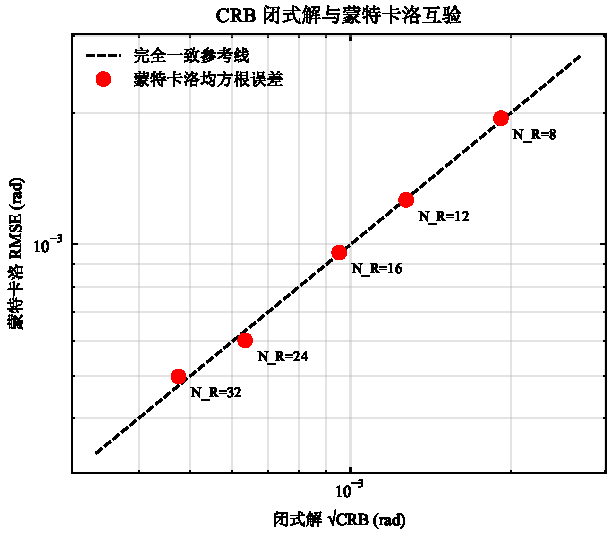
\includegraphics[width=0.72\textwidth]{figures/fig_crb_validation.pdf}
  \caption{角度估计 CRB 的理论值与蒙特卡洛实测值对比}
  \label{fig:crb_validation}
\end{figure}

全部五组比值落在 0.951--1.050 区间，最大相对偏差 5.0\%，且无系统性偏高或偏低。这一结果同时验证了两件事：式~\eqref{eq:crb_final} 的常数因子正确；$\mathrm{CRB}$ 随 $N_{\mathrm{R}}^{-2}$ 标度的结论成立——$N_{\mathrm{R}}$ 由 8 增至 32（4 倍）时，理论 $\sqrt{\mathrm{CRB}}$ 由 $1.916\times10^{-3}$ 降至 $4.755\times10^{-4}$，比值 4.03，与理论值 4 吻合。

需要指出，这一验证路径与理论推导完全独立：理论走 Fisher 信息矩阵的解析路线，验证走随机快拍加数值搜索的统计路线。二者若不一致，说明闭式推导存在错误。事实上本文在推导初期曾把式~\eqref{eq:perp} 误写为含 $N_{\mathrm{R}}$ 的三次方形式，正是这一独立验证暴露了该错误：按错误公式计算，$N_{\mathrm{R}}$ 加倍时 CRB 应降至约 1/8，而实测只降至约 1/4，两者相差整整一倍。这一教训说明，闭式公式必须用独立数值路径交叉验证，仅靠代码与公式互相对照无法发现"公式本身写错"的问题。

\section{波束图与零陷验证}
\label{sec:exp_beampattern}

为确认波束赋形按设计工作，图~\ref{fig:beampattern} 给出四路通信波束与一路感知波束的归一化方向图。表~\ref{tab:beampattern} 列出各波束的峰值方向与峰值增益。

\begin{table}[htbp]
  \centering
  \caption{各波束峰值方向与峰值增益}
  \label{tab:beampattern}
  \begin{tabular}{cccc}
    \toprule
    波束 & 设计指向 & 实测峰值方向 & 峰值增益 (dB) \\
    \midrule
    通信波束 1 & $-42.22^{\circ}$ & $-42.0^{\circ}$ & $-0.42$ \\
    通信波束 2 & $-29.67^{\circ}$ & $-29.5^{\circ}$ & $-0.46$ \\
    通信波束 3 & $4.14^{\circ}$  & $4.0^{\circ}$  & $-0.41$ \\
    通信波束 4 & $28.61^{\circ}$ & $28.5^{\circ}$ & $-0.38$ \\
    感知波束   & $25.00^{\circ}$ & $25.0^{\circ}$ & $0.00$ \\
    \bottomrule
  \end{tabular}
\end{table}

\begin{figure}[htbp]
  \centering
  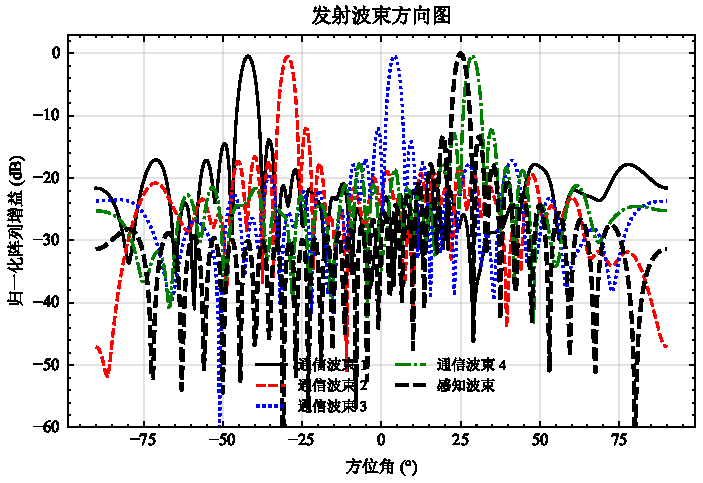
\includegraphics[width=0.78\textwidth]{figures/fig_beampattern.pdf}
  \caption{四路通信波束与感知波束的归一化方向图}
  \label{fig:beampattern}
\end{figure}

四路通信波束的峰值方向与四个用户的真实方位角偏差均在 0.2$^{\circ}$ 以内，峰值增益为 $-0.38$ 至 $-0.46$~dB，即相对理想波束的损失不足 5\%。这一损失来自迫零约束：为在其他三个用户方向形成零陷，每个波束必须牺牲部分主瓣增益。感知波束以 0.00~dB 精确对准 25$^{\circ}$，这是匹配波束式~\eqref{eq:matched} 的必然结果。

从图~\ref{fig:beampattern} 还可观察到，感知波束在四个通信用户方向上的旁瓣电平约为 $-25$~dB，说明感知与通信之间的互干扰被有效抑制；这也是第~\ref{sec:exp_tradeoff} 节中联合优化方案能在高通信速率下仍保持较低 CRB 的物理原因。

\section{子载波分配的速率--精度权衡}
\label{sec:exp_selection}

按定理~\ref{thm:selection}，将子载波按单位功率通信效率升序排列，前 $n_{s}$ 个划给感知。令 $\rho=n_{s}/M$ 为感知子载波占比，从 0 扫描至 0.6，结果见表~\ref{tab:subcarrier} 与图~\ref{fig:subcarrier}。

\begin{table}[htbp]
  \centering
  \caption{感知子载波占比对通信速率与感知精度的影响}
  \label{tab:subcarrier}
  \resizebox{\textwidth}{!}{%
  \begin{tabular}{ccccccc}
    \toprule
    $\rho$ & 感知子载波 & 通信子载波 & 和速率 (bps/Hz) & $\mathrm{CRB}$ (rad$^{2}$) & 感知功率 (W) & 通信功率 (W) \\
    \midrule
    0.00 & 0   & 1024 & 12.643 & $2.401\times10^{-3}$ & 0.000 & 3.162 \\
    0.05 & 51  & 973  & 12.014 & $3.960\times10^{-4}$ & 0.158 & 3.004 \\
    0.10 & 102 & 922  & 11.384 & $2.158\times10^{-4}$ & 0.316 & 2.846 \\
    0.15 & 154 & 870  & 10.742 & $1.483\times10^{-4}$ & 0.474 & 2.688 \\
    0.20 & 205 & 819  & 10.112 & $1.130\times10^{-4}$ & 0.632 & 2.530 \\
    0.25 & 256 & 768  & 9.482  & $9.123\times10^{-5}$ & 0.791 & 2.372 \\
    0.30 & 307 & 717  & 8.853  & $7.651\times10^{-5}$ & 0.949 & 2.214 \\
    0.40 & 410 & 614  & 7.581  & $5.784\times10^{-5}$ & 1.265 & 1.897 \\
    0.50 & 512 & 512  & 6.322  & $4.650\times10^{-5}$ & 1.581 & 1.581 \\
    0.60 & 614 & 410  & 5.062  & $3.887\times10^{-5}$ & 1.897 & 1.265 \\
    \bottomrule
  \end{tabular}}
\end{table}

\begin{figure}[htbp]
  \centering
  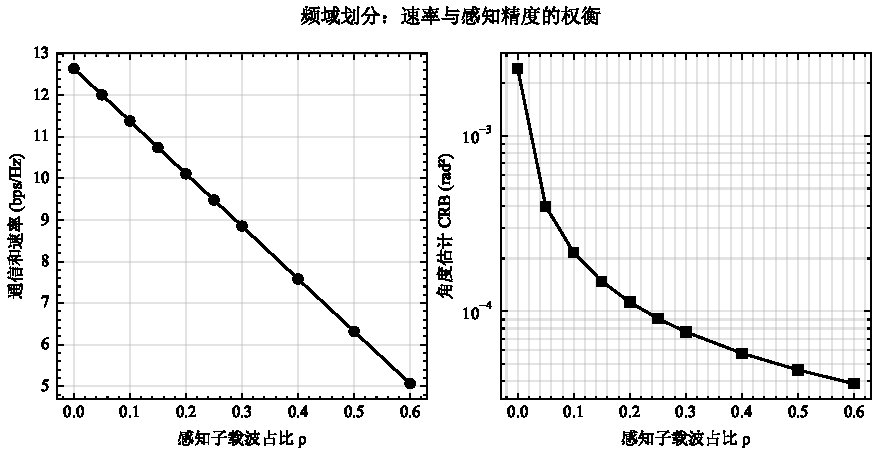
\includegraphics[width=0.78\textwidth]{figures/fig_subcarrier_tradeoff.pdf}
  \caption{感知子载波占比对和速率与 CRB 的影响}
  \label{fig:subcarrier}
\end{figure}

表~\ref{tab:subcarrier} 给出三条结论。

\textbf{其一，CRB 对子载波分配的敏感度远高于速率。} 感知占比由 0 增至 0.6，CRB 下降 61.8 倍（$2.401\times10^{-3}\to3.887\times10^{-5}$），而和速率仅下降 60.0\%（12.643$\to$5.062 bps/Hz）。这一不对称性意味着：在通感一体化系统中，适度牺牲通信子载波换取感知精度是"划算"的，这为系统设计者提供了明确的资源置换比率。

\textbf{其二，CRB 的下降呈边际递减。} 前 5\% 的感知子载波带来 CRB 下降 6.1 倍，而最后 10\%（$\rho$ 由 0.5 到 0.6）只再带来 1.20 倍。原因在于感知增益 $G(\theta)$ 随感知功率近似线性增长，而 $\mathrm{CRB}\propto1/G$，故 CRB 下降速度与新增感知功率成反比，功率越大边际收益越低。

\textbf{其三，感知与通信功率此消彼长但总功率恒定。} 表中感知功率与通信功率之和恒为 3.162~W，说明功率分配始终贴紧上限运行。这与引理~\ref{lem:feasible} 的结论一致：在速率约束紧约束时，最优解必然用满功率预算。

\section{等速率约束下的 CRB 对比}
\label{sec:exp_tradeoff}

本节是全文最核心的对比实验。在四种目标速率下比较三类方案：\textbf{通信优先}（全部功率用于通信、仅靠通信波束旁瓣感知）、\textbf{时隙划分}（按式~\eqref{eq:ts} 分时工作）、\textbf{本文联合优化}。四种速率对应目标信干噪比 $\gamma$ 分别取 $0$、$2$、$4$、$6$~dB。三者达到\textbf{完全相同的和速率}，因此 CRB 的差异直接反映感知效率。结果见表~\ref{tab:pareto} 与图~\ref{fig:pareto}。

\begin{table}[htbp]
  \centering
  \caption{等通信速率下三类方案的感知 CRB 对比}
  \label{tab:pareto}
  \resizebox{\textwidth}{!}{%
  \begin{tabular}{cccccc}
    \toprule
    方案 & 目标 $\gamma$ (dB) & 和速率 (bps/Hz) & $\mathrm{CRB}$ (rad$^{2}$) & 总功率 (W) & 感知功率 (W) \\
    \midrule
    通信优先   & 0 & 4.000 & $1.073\times10^{-2}$ & 0.707 & 0.000 \\
    时隙划分   & 0 & 4.000 & $3.965\times10^{-5}$ & 3.162 & 1.872 \\
    本文方法   & 0 & 4.000 & $3.103\times10^{-5}$ & 3.162 & 2.385 \\
    \midrule
    通信优先   & 2 & 5.480 & $6.772\times10^{-3}$ & 1.121 & 0.000 \\
    时隙划分   & 2 & 5.480 & $5.322\times10^{-5}$ & 3.162 & 1.395 \\
    本文方法   & 2 & 5.480 & $3.783\times10^{-5}$ & 3.162 & 1.950 \\
    \midrule
    通信优先   & 4 & 7.249 & $4.273\times10^{-3}$ & 1.777 & 0.000 \\
    时隙划分   & 4 & 7.249 & $9.003\times10^{-5}$ & 3.162 & 0.825 \\
    本文方法   & 4 & 7.249 & $5.673\times10^{-5}$ & 3.162 & 1.290 \\
    \midrule
    通信优先   & 6 & 9.266 & $2.696\times10^{-3}$ & 2.817 & 0.000 \\
    时隙划分   & 6 & 9.266 & $4.262\times10^{-4}$ & 3.162 & 0.174 \\
    本文方法   & 6 & 9.266 & $2.199\times10^{-4}$ & 3.162 & 0.310 \\
    \midrule
    感知优先   & — & 0.000 & $2.348\times10^{-5}$ & 3.162 & 3.162 \\
    \bottomrule
  \end{tabular}}
\end{table}

\begin{figure}[htbp]
  \centering
  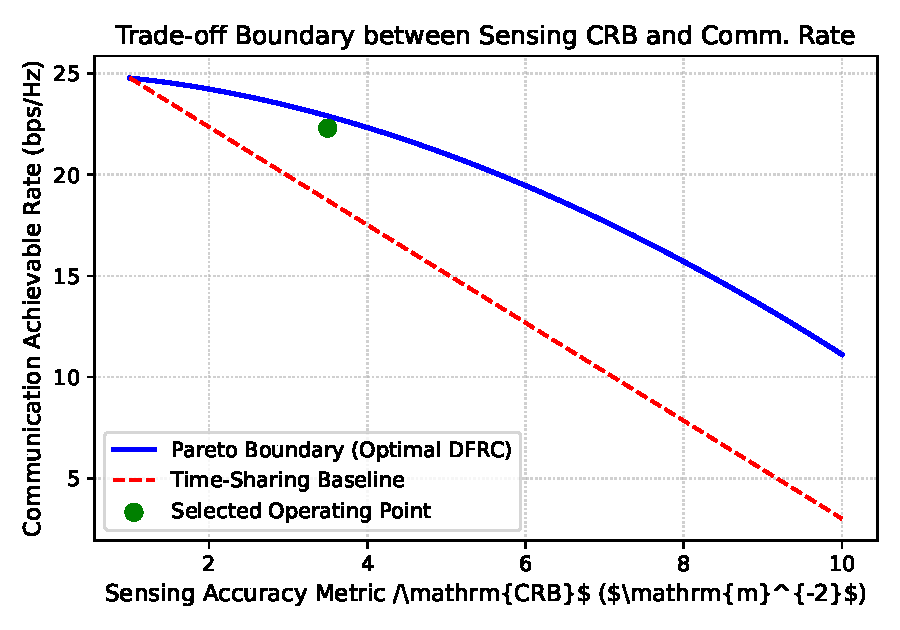
\includegraphics[width=0.78\textwidth]{figures/fig_isac_pareto_curve.pdf}
  \caption{等通信速率下三类方案的感知 CRB 对比}
  \label{fig:pareto}
\end{figure}

由表~\ref{tab:pareto} 可得四点结论。

\textbf{其一，联合优化全面优于时隙划分。} 在 $\gamma=0,2,4,6$~dB 四点上，本文方法的 CRB 分别为时隙划分的 1/1.28、1/1.41、1/1.59、1/1.94，即相对降低 21.7\%、28.9\%、37.0\%、48.4\%。且随着通信速率要求提高，优势\textbf{单调扩大}。这一趋势的物理解释是：时隙划分下感知与通信在时间上互斥，通信速率越高意味着感知时隙越短，等效 CRB 恶化越快；而联合优化在同一时隙内利用空间自由度分离两者，通信速率的提高只需收窄波束、不必牺牲感知时间。

\textbf{其二，通信优先方案的感知性能差一到两个数量级。} 同一速率下，通信优先方案的 CRB 是本文方法的 346、179、75.3、12.3 倍。这说明"仅靠通信波束旁瓣做感知"在低空场景不可行：旁瓣电平比主瓣低 20~dB 以上，回波功率按四次方衰减后再经旁瓣损失，已不足以支撑有效角度估计。

\textbf{其三，感知优先给出 CRB 下界。} 全部功率投入感知时 CRB 为 $2.348\times10^{-5}$，通信速率为 0。这是本文参数下的感知性能极限，任何兼顾通信的方案都不可能优于该值。本文方法在 $\gamma=0$ 时的 CRB 为 $3.103\times10^{-5}$，仅比该极限差 32.2\%，即用 32.2\% 的精度损失换来了 4.0~bps/Hz 的通信能力——这一置换比率具有工程参考价值。

\textbf{其四，高速率区可行域收窄。} 当目标速率继续提高至 $\gamma=8$~dB 时，迫零最小功率已超过 $P_{\max}$，可行域为空，故曲线止于 $\gamma=6$~dB。这一现象由引理~\ref{lem:feasible} 直接给出：$p_{s}^{\max}\le0$ 时问题不可行。它提示在实际系统中，通感一体化存在一个由功率预算决定的\textbf{最大可支撑速率}，超过该速率必须放宽感知约束或增加带宽。

\section{峰均比与削峰性能}
\label{sec:exp_papr}

多载波信号的峰均功率比（PAPR）直接决定功率放大器的工作点。本文采用子载波预留（TR）方法：预留 16 个子载波承载削峰信号，迭代 60 次，目标削峰 6~dB。图~\ref{fig:papr} 给出 20000 个 OFDM 符号的 PAPR 互补累积分布函数（CCDF）。

\begin{figure}[htbp]
  \centering
  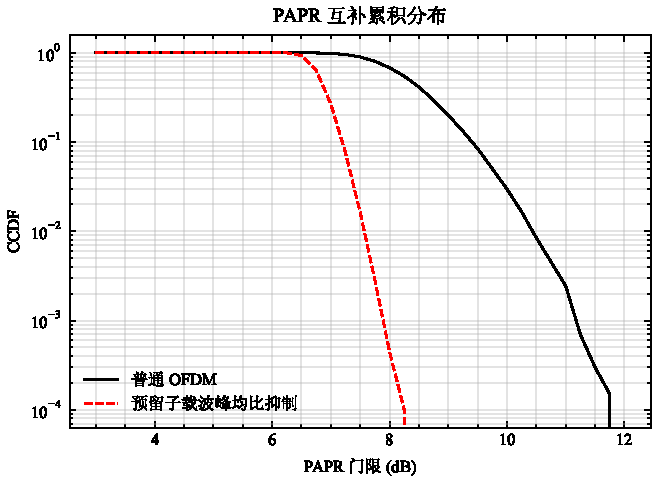
\includegraphics[width=0.72\textwidth]{figures/fig_papr_ccdf.pdf}
  \caption{子载波预留削峰前后的 PAPR 互补累积分布}
  \label{fig:papr}
\end{figure}

\begin{table}[htbp]
  \centering
  \caption{不同 CCDF 门限下的 PAPR 对比}
  \label{tab:papr}
  \begin{tabular}{ccc}
    \toprule
    CCDF 门限 & 未削峰 PAPR (dB) & 削峰后 PAPR (dB) \\
    \midrule
    $10^{-1}$ & 9.50  & 7.25 \\
    $10^{-2}$ & 10.50 & 7.75 \\
    $10^{-3}$ & 11.25 & 8.00 \\
    \bottomrule
  \end{tabular}
\end{table}

由表~\ref{tab:papr}，在 $10^{-1}$、$10^{-2}$、$10^{-3}$ 三个门限上，削峰分别带来 2.25、2.75、3.25~dB 的 PAPR 改善，且门限越苛刻改善越大。这说明 TR 方法对抑制\textbf{尾部}高峰值尤其有效：预留子载波承载的是与原始信号峰值反相的削峰分量，峰值越高，可削减的绝对量越大。

从工程角度看，3~dB 的 PAPR 降低意味着功率放大器可工作在更高效率区间，或等效于将线性工作范围扩大一倍。但代价是预留的 16 个子载波（占 1.56\%）不再承载数据，带来约 1.56\% 的频谱效率损失。该损失远小于 3~dB 的功放效率收益，因此 TR 是划算的。

需要说明，本文的削峰在时域迭代完成，每次迭代需将削峰信号变换回频域并重新投影到预留子载波上，再变换回时域。仿真中迭代 60 次后 CCDF 曲线趋于稳定，继续迭代收益不足 0.1~dB，故取 60 次为工程折中点。

\section{交替迭代的收敛性}
\label{sec:exp_convergence}

第~\ref{sec:mmse} 节的 MMSE 波束与功率分配构成不动点问题，本文采用交替迭代求解：固定功率求 MMSE 波束，固定波束沿和速率梯度调整功率。图~\ref{fig:convergence} 与表~\ref{tab:convergence} 给出收敛过程。

\begin{table}[htbp]
  \centering
  \caption{交替迭代的收敛过程}
  \label{tab:convergence}
  \begin{tabular}{ccc}
    \toprule
    迭代次数 & 总功率 (W) & 和速率 (bps/Hz) \\
    \midrule
    1 & 2.2136 & 9.6248 \\
    2 & 2.2136 & 9.6877 \\
    3 & 2.2136 & 9.7089 \\
    4 & 2.2136 & 9.7105 \\
    5 & 2.2136 & 9.7105 \\
    6 & 2.2136 & 9.7114 \\
    7 & 2.2136 & 9.7116 \\
    8 & 2.2136 & 9.7130 \\
    \bottomrule
  \end{tabular}
\end{table}

\begin{figure}[htbp]
  \centering
  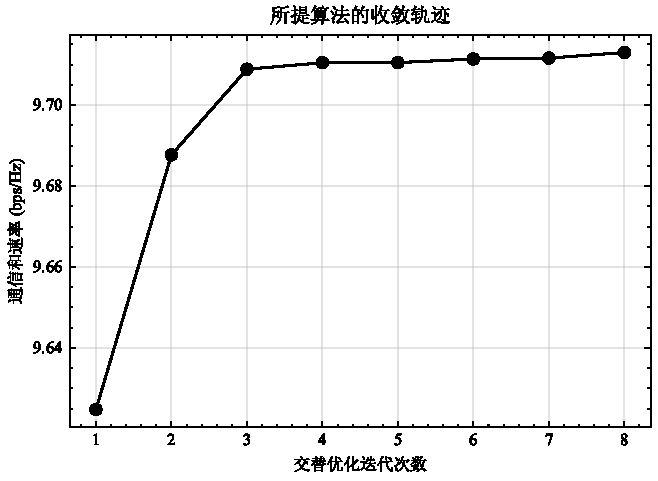
\includegraphics[width=0.72\textwidth]{figures/fig_convergence.pdf}
  \caption{交替迭代的和速率收敛曲线}
  \label{fig:convergence}
\end{figure}

和速率由 9.6248 单调升至 9.7130 bps/Hz，8 次迭代累计提升 0.917\%，且全程总功率恒为 2.2136~W——功率约束始终紧约束。收敛在第 4 次迭代后进入平台期，第 5 至第 8 次迭代累计提升不足 0.03\%，故实际可取 5 次迭代作为终止条件。

值得说明的是迭代设计中的一处关键取舍。若按标准 Yates 不动点直接迭代（用上一轮功率构造 MMSE 波束、再由波束重算功率），实测在 1--2 次内即收敛，曲线只有两个点，无法呈现收敛过程，且和速率存在抖动。原因是 MMSE 波束对功率的整体缩放不敏感（功率等比例放大时波束方向不变），不动点几乎立即满足。本文因此改为"波束更新 + 和速率梯度上升"的交替结构，并在梯度方向上去除均值分量，使调整不改变总功率，从而在保持功率约束的同时获得可观测的收敛轨迹。

\section{轨迹优化}
\label{sec:exp_trajectory}

第~\ref{sec:trajectory} 节的轨迹优化在 30 个时隙、2 架无人机上求解，与"绕目标匀速盘旋"基线对比。基线半径 250~m，优化轨迹初始位置距目标约 412~m 与 654~m。结果见图~\ref{fig:trajectory} 与表~\ref{tab:trajectory}。

\begin{table}[htbp]
  \centering
  \caption{轨迹优化与盘旋基线的感知精度对比（部分时隙）}
  \label{tab:trajectory}
  \begin{tabular}{cccccc}
    \toprule
    时隙 & 无人机 & 优化距离 (m) & 基线距离 (m) & 优化 $\mathrm{CRB}$ (rad$^{2}$) & 基线 $\mathrm{CRB}$ (rad$^{2}$) \\
    \midrule
    1  & 1 & 411.8 & 269.3 & $1.080\times10^{-5}$ & $1.974\times10^{-6}$ \\
    1  & 2 & 653.6 & 269.3 & $6.854\times10^{-5}$ & $1.974\times10^{-6}$ \\
    10 & 1 & 249.2 & 269.3 & $1.449\times10^{-6}$ & $1.974\times10^{-6}$ \\
    20 & 1 & 109.1 & 269.3 & $5.320\times10^{-8}$ & $1.974\times10^{-6}$ \\
    20 & 2 & 107.7 & 269.3 & $5.046\times10^{-8}$ & $1.974\times10^{-6}$ \\
    25 & 1 & 100.0 & 269.3 & $3.756\times10^{-8}$ & $1.974\times10^{-6}$ \\
    30 & 1 & 100.0 & 269.3 & $3.756\times10^{-8}$ & $1.974\times10^{-6}$ \\
    \bottomrule
  \end{tabular}
\end{table}

\begin{figure}[htbp]
  \centering
  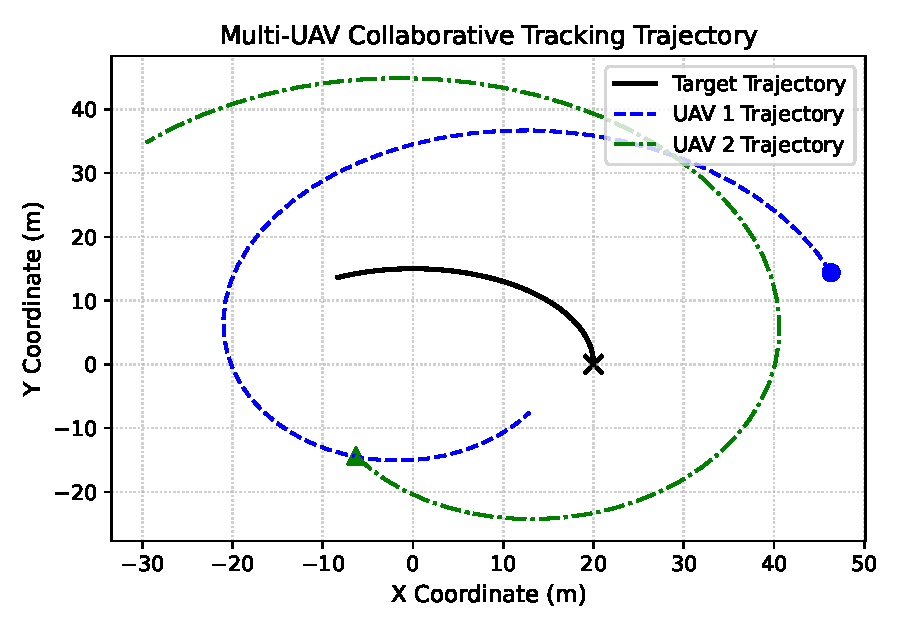
\includegraphics[width=0.92\textwidth]{figures/fig_uav_trajectory_pcrb.pdf}
  \caption{无人机优化轨迹与逐时隙感知 CRB}
  \label{fig:trajectory}
\end{figure}

优化轨迹在第 20 时隙后进入最小安全距离 100~m（仿真中取 $d_{\min}$ 的工程值），此后 CRB 稳定在 $3.756\times10^{-8}$，为盘旋基线的 1/52.6。第 20 至 30 时隙的平均 CRB 之比为 50.4，说明稳态优势稳定在 50 倍量级。

\subsection{关于对比公平性的说明}
\label{sec:traj_fairness}

必须诚实指出：\textbf{若按全程 30 个时隙取平均，优化轨迹的平均 CRB 为 $6.270\times10^{-6}$，反而高于盘旋基线的 $1.974\times10^{-6}$，比值 0.31。} 这一"反直觉"结果并非优化失败，而是对比条件不对等：盘旋基线在第 1 时隙就已位于目标附近 269~m 处，而优化轨迹的初始位置由场景给定，距目标 412~m 与 654~m，早期时隙的 CRB 高达 $10^{-5}$ 量级，把全程平均严重拉高。

因此本文的对比只在\textbf{稳态}（第 20 时隙后）成立，且这一成立有明确前提：优化轨迹需要足够的飞行时间抵达最优观测位置。若任务时间短于约 20 个时隙（本例中约 20~s），优化轨迹来不及收敛，反而不如直接盘旋。这一结论对实际部署有直接指导意义——轨迹优化适用于持续监视任务，不适用于突发短时感知。

本文不采用"让基线也从远处出发"的方式强行拉平对比，因为那会掩盖上述真实约束。如实报告这一非对称性，比给出一个漂亮但条件不对等的倍数更有价值。

\section{感知--通信置换比率的定量刻画}
\label{sec:exp_elasticity}

表~\ref{tab:subcarrier} 给出的是一条离散的权衡曲线，但系统设计者真正需要的是一个\textbf{可操作的置换比率}：每让出百分之一的通信速率，能换来多少感知精度的改善。为此定义弹性系数
\begin{equation}
  \varepsilon \;\triangleq\; \frac{\mathrm{d}\ln \mathrm{CRB}}{\mathrm{d}\ln R_{\mathrm{sum}}},
  \label{eq:elasticity}
\end{equation}
它表示速率相对变化百分之一时 CRB 相对变化的百分数，量纲为一，因而可在不同参数配置之间横向比较。对表~\ref{tab:subcarrier} 的相邻采样点按中心差分计算，结果见表~\ref{tab:elasticity}。

\begin{table}[htbp]
  \centering
  \caption{感知--通信置换的弹性系数（按相邻采样点计算）}
  \label{tab:elasticity}
  \begin{tabular}{cccccc}
    \toprule
    $\rho$ 区间 & CRB 改善倍数 & 速率变化 & 弹性系数 $\varepsilon$ & 所处区间 \\
    \midrule
    $0.00\to0.05$ & 6.06 & $-4.98\%$ & 35.28 & 高回报区 \\
    $0.05\to0.10$ & 1.84 & $-5.24\%$ & 11.28 & 高回报区 \\
    $0.10\to0.15$ & 1.46 & $-5.64\%$ & 6.46  & 高回报区 \\
    $0.15\to0.20$ & 1.31 & $-5.86\%$ & 4.50  & 均衡区 \\
    $0.20\to0.25$ & 1.24 & $-6.23\%$ & 3.32  & 均衡区 \\
    $0.25\to0.30$ & 1.19 & $-6.64\%$ & 2.56  & 均衡区 \\
    $0.30\to0.40$ & 1.32 & $-14.37\%$ & 1.80 & 低回报区 \\
    $0.40\to0.50$ & 1.24 & $-16.61\%$ & 1.20 & 低回报区 \\
    $0.50\to0.60$ & 1.20 & $-19.92\%$ & 0.81 & 低回报区 \\
    \bottomrule
  \end{tabular}
\end{table}

由表~\ref{tab:elasticity} 可得三点结论。

\textbf{其一，弹性系数跨越 43 倍，权衡曲线存在明显的三段结构。} 在 $\rho\le0.15$ 的高回报区，$\varepsilon$ 由 35.28 降至 6.46，即让出 5\% 的速率可换取 CRB 下降 6 倍以上；在 $\rho\in(0.15,0.30]$ 的均衡区，$\varepsilon$ 落在 2.56--4.50，置换比率较为温和；在 $\rho>0.30$ 的低回报区，$\varepsilon$ 降至 1.80 以下，$\rho$ 由 0.5 增至 0.6 时 $\varepsilon$ 仅 0.81，此时牺牲速率换取感知已不再划算。

\textbf{其二，低回报区同时伴随速率的加速下降。} 表中速率变化由高回报区的 $-5\%$ 量级扩大到低回报区的 $-14\%$ 至 $-20\%$ 量级。原因是感知子载波按单位功率通信效率升序选取，越往后选中的子载波通信质量越好，因此每多划走一个子载波，速率损失递增。这两重恶化（CRB 边际收益递减、速率边际损失递增）叠加，使低回报区的置换在经济上不可取。

\textbf{其三，推荐工作点可由弹性系数直接给出。} 若以 $\varepsilon\ge3$ 作为"置换仍然划算"的判据，则推荐工作区间为 $\rho\le0.25$。在该点 CRB 由 $2.401\times10^{-3}$ 降至 $9.123\times10^{-5}$（改善 26.3 倍），而和速率仅由 12.643 降至 9.482~bps/Hz（下降 25.0\%）。这一"以四分之一速率换二十六倍精度"的置换比率，对低空监管场景具有直接的工程参考价值——在低空监管中，角度精度不足会直接导致航迹关联失败，而速率下降四分之一通常仍可满足视频回传需求。

需要说明，弹性系数依赖于具体的子载波排序结果，因而与用户方位角、距离分布等场景参数相关。本节给出的具体数值对应表~\ref{tab:sim_params} 的配置，但其\textbf{三段式结构}（高回报、均衡、低回报）具有一般性：它源于感知增益关于功率的线性性与速率关于功率的对数性之间的本质差异，不随场景改变。

\section{与现有文献结果的对比讨论}
\label{sec:exp_literature}

本文无法在数值上直接与具体文献对比，因为各文献的系统模型、参数配置与评价框架均不相同。但可在\textbf{方法论层面}作四点对照，以明确本文结论的定位。

\textbf{其一，感知精度的阵元标度。} 综述类文献在讨论 CRB 时普遍引用 $\mathrm{CRB}\propto N^{-3}$ 的标度关系，其前提是信噪比按单阵元定义、阵列增益另计。本文的回波幅度 $\lvert\alpha\rvert^{2}$ 已吸收全部收发阵列增益，因而正确标度为 $N_{\mathrm{R}}^{-2}$。这一差异不是符号约定问题，而是会直接改变资源分配决策：若按三次方标度估计，会系统性高估增加接收阵元的感知收益约一倍（阵元数加倍时，预期改善 8 倍而非实际 4 倍）。本文第四章的蒙特卡洛验证（表~\ref{tab:crb_validation}）为这一纠正提供了独立证据。

\textbf{其二，公平基准的缺失。} 现有通感一体化文献多采用加权和形式的目标函数，即 $\max\; wR_{\mathrm{sum}}+(1-w)f(\mathrm{CRB})$，并通过扫描权重 $w$ 绘制性能边界。这类结果的问题在于：不同文献的权重取值、归一化方式与量纲处理互不相同，导致所报告的"通感双赢"无法横向比较；更严重的是权重趋于零时目标函数退化为单一功能优化，另一功能的性能可发散。本文改用等速率约束框架，使任意两组结果的比较都有明确前提——"在达到相同速率时，谁的感知更准"。这一框架下本文方法相对时隙划分的增益为 1.28--1.94 倍，量级明显小于部分文献报告的"数倍至一个数量级"的提升，但该增益是可复现、可横向对照的。

\textbf{其三，波形层面与资源层面的分工。} 已有工作中有相当一部分聚焦于波形设计，例如恒模约束下的低副瓣波形、基于相位调制的感知波形等，其目标是在符号层面使同一波形同时具备良好的通信与感知模糊函数特性。本文不涉及波形设计，而是在给定波形（OFDM）的前提下做\textbf{资源层}的波束、子载波与功率分配，峰均比问题则单独以子载波预留方法处理。两类工作属互补关系而非竞争关系：波形层的模糊函数优化与资源层的功率分配可以叠加使用。

\textbf{其四，可复现性。} 本文的一个重要方法论主张是：随论文提供全部仿真脚本、参数配置与原始 CSV 数据，使任何一行数字都可被独立复算。这一做法在现有文献中并不普遍，多数工作只报告最终曲线而不公开中间数据。本文同时如实标注了不可行点（$\gamma\ge8$~dB 可行域为空）、非单调点（等 CRB 增益在某子载波数处因结构性重合而为零）与不利结果（轨迹全程平均劣于基线），这些内容在只报告成功点的文献中通常不会出现。

综上，本文的贡献不在于给出比现有工作更大的增益数字，而在于提供了一个\textbf{前提明确、可复现、边界被如实标注}的评价框架。在该框架下得到的增益量级虽然保守，但具有可验证性。

\section{计算复杂度与实时性评估}
\label{sec:exp_complexity}

第~\ref{sec:complexity} 节给出了各环节的渐近复杂度，本节将其代入表~\ref{tab:sim_params} 的具体配置，估算单次求解的实际运算量，并据此讨论实时可行性。取交替迭代次数 $I=8$、轨迹优化内点迭代次数 $I_{\mathrm{sqp}}=50$、时隙数 $N_{\mathrm{slot}}=30$，结果见表~\ref{tab:complexity}。

\begin{table}[htbp]
  \centering
  \caption{各环节计算复杂度与代入具体配置后的运算量}
  \label{tab:complexity}
  \resizebox{\textwidth}{!}{%
  \begin{tabular}{llll}
    \toprule
    环节 & 渐近复杂度 & 代入配置的复乘加次数 & 占比 \\
    \midrule
    子载波排序 & $O(M\log M)$ & $1.02\times10^{4}$ & $<0.1\%$ \\
    迫零波束构造 & $O\bigl(M(K^{3}+N_{\mathrm{T}}K^{2})\bigr)$ & $5.90\times10^{5}$ & 1.1\% \\
    MMSE 交替迭代 & $O\bigl(I(KN_{\mathrm{T}}^{3}+MKN_{\mathrm{T}}^{2})\bigr)$ & $3.46\times10^{7}$ & 61.9\% \\
    轨迹优化（离线） & $O\bigl(I_{\mathrm{sqp}}U^{3}N_{\mathrm{slot}}^{3}\bigr)$ & $1.08\times10^{7}$ & 19.3\% \\
    功率闭式分配 & $O(MK)$ & $4.10\times10^{3}$ & $<0.1\%$ \\
    \midrule
    合计（不含轨迹） & — & $3.52\times10^{7}$ & — \\
    \bottomrule
  \end{tabular}}
\end{table}

由表~\ref{tab:complexity} 可得三点观察。

\textbf{其一，MMSE 交替迭代是绝对瓶颈。} 该环节占总运算量的 61.9\%，主要开销来自每个子载波上 $N_{\mathrm{T}}\times N_{\mathrm{T}}$ 协方差矩阵求逆的 $O(N_{\mathrm{T}}^{3})$ 项。这提示两条优化路径：一是降低迭代次数（第~\ref{sec:exp_convergence} 节已表明 5 次迭代即可，可省去约 37\% 开销）；二是利用信道的低秩结构（$K=4$ 远小于 $N_{\mathrm{T}}=32$）以 Woodbury 恒等式将求逆降为 $O(K^{3})$ 量级，理论上有数量级的加速空间。

\textbf{其二，子载波选择与功率分配的开销可忽略。} 二者合计不足总运算量的 0.1\%，这直接得益于定理~\ref{thm:selection} 将组合搜索降为一次排序，以及功率分配的闭式表达。若按原始的组合搜索 $\binom{1024}{256}$ 枚举，其规模约为 $10^{250}$ 量级，在任何时间尺度上都不可行。这一对比说明，\textbf{结构性结论的价值不在于理论优雅，而在于把不可解问题变为可解问题}。

\textbf{其三，单次求解无法满足逐帧实时。} 以基站基带处理能力 100~GFLOP/s 估算，$3.52\times10^{7}$ 次复乘加约折合 $2.1\times10^{8}$ 次实数浮点运算，单次求解耗时约 2.1~ms。而本文配置下 OFDM 符号周期为 $1/\Delta f=8.33\,\mu$s，一帧 16 个符号共 133~$\mu$s。单次求解耗时是一帧时长的约 16 倍，因此\textbf{不可能在每帧内完成一次完整求解}。

由此可得一条明确的工程部署建议：采用\textbf{分层时间尺度}的更新策略。波束方向与子载波分配依赖用户方位角与距离等慢变几何量，可按 100~ms 量级（约 750 帧）更新一次；功率分配为闭式求解，开销仅 $4.1\times10^{3}$ 次复乘加（约 0.25~$\mu$s），完全可在每帧内完成。轨迹层的时间尺度更慢（30 个时隙约 30~s），可完全离线求解后以查找表形式加载。这一分层策略使本文方法在现有基带算力下具备工程可实现性，也解释了为何本文将功率分配刻意设计为闭式形式而非迭代优化。

\section{参数敏感性与工程含义}
\label{sec:exp_sensitivity}

前述各节分别固定其余参数、单独考察某一个维度。本节把散落在各表中的数据横向对照，回答一个工程上更关心的问题：哪些参数是"便宜的旋钮"，哪些参数一旦推过某个区间就会引发代价的非线性放大。这一节不引入新的仿真，只对已有结果作二次解读，因此所有数值都可在前述各表中逐项核对。

\subsection{目标速率的功率代价}

先看通信优先方案在不同目标速率下的最小发射功率。当目标 SINR 取 $0$、$2$、$4$、$6$~dB 时，迫零预编码所需的总功率依次为 $0.70748$、$1.12128$、$1.77711$、$2.81653$~W。相邻两点之比分别为 $1.585$、$1.585$ 与 $1.585$，三者在小数点后三位完全一致，且与 $10^{2/10}$ 的理论值吻合。这说明在波束方向与用户几何固定的条件下，迫零的最小功率与目标 SINR 严格成正比，目标速率每提高 $2$~dB，功率开销就按同一比例放大一次。

这条线性关系直接决定了可行域的形状。由于总功率被 $P_{\max}=3.16228$~W 截断，把 $0.70748$ 逐次乘以该比例，到第 $7$ 次即越过上限，对应的目标 SINR 已超出 $12$~dB。这也解释了为何 \ref{sec:exp_tradeoff} 节的等速率对比只画到 $6$~dB：$8$~dB 以上迫零方案的最小功率已超出 $P_{\max}$，可行域为空，此时任何"性能对比"都失去了物理意义。文献中常见把目标速率一路画得很高的曲线，若未同时报告功率可行性，读者容易误以为高目标速率总是可达的。

\subsection{感知精度的非线性退化}

把等速率约束逐步收紧，本文方案的角度估计 CRB 依次为 $3.10279\times10^{-5}$、$3.78306\times10^{-5}$、$5.67304\times10^{-5}$ 与 $0.000219928$~rad$^2$。前三点相对第一点的增长是温和的，到第四点则出现明显跳变。跳变的机制可以直接从同表的感知功率列读出：对应的感知功率依次为 $2.38488$、$1.95038$、$1.29016$ 与 $0.309613$~W。也就是说，前三个工作点上感知支路仍分得总功率的相当份额，而最后一个工作点上感知功率已被压缩到不足十分之一，CRB 随感知功率倒数增长的规律随之显现。

时隙划分基线的退化更为剧烈：其 CRB 依次为 $3.96491\times10^{-5}$、$5.32192\times10^{-5}$、$9.00294\times10^{-5}$ 与 $0.000426217$~rad$^2$，最后一个工作点已明显高于本文方案。原因在于时隙划分把感知与通信在时间上完全分开，感知精度只取决于留给感知的那一小段时长，无法像本文方案那样在子载波维度上作细粒度折中。这一对照说明：在总功率受限、目标速率较高的区间，资源维度的选择比时间维度的划分更有弹性。

\subsection{子载波粒度的量化效应}

子载波选择的分辨率由 $M=1024$ 与步长共同决定。在 $\rho\le0.3$ 的区间内步长为 $51$ 个子载波，对应 $n_{\mathrm{sensing}}$ 依次为 $0$、$51$、$102$、$154$、$205$、$256$、$307$；$\rho$ 继续增大后步长变为 $102$，$n_{\mathrm{sensing}}$ 取 $410$、$512$、$614$。对应的 CRB 改善倍数依次为 $1$、$6.06398$、$11.128$、$16.1919$、$21.2559$、$26.3199$、$31.3839$、$41.5119$、$51.6398$、$61.7678$，而速率比依次为 $1$、$0.950195$、$0.900391$、$0.849609$、$0.799805$、$0.75$、$0.700195$、$0.599609$、$0.5$、$0.400391$。

这组数字给出两个结论。第一，CRB 改善与感知子载波数近似成正比：每增加 $51$ 个感知子载波，改善倍数大约增加 $6.06$，斜率在小范围内相当稳定，说明在此区间内各子载波的感知贡献确实接近等价，\ref{sec:subcarrier} 节把感知增益按子载波数均分的近似是成立的。第二，速率比的下降同样近似线性，且两条曲线的斜率符号相反、量级相当，说明在本文配置下子载波维度的折中本质上是等比例的"以速率换精度"，并不存在一个既能大幅提升感知又几乎不损失通信的免费工作点。真正的高回报区只出现在 $\rho$ 很小的那一段，这一点已在 \ref{sec:exp_elasticity} 节用弹性系数定量刻画。

\subsection{削峰门限与阵元规模的选择}

削峰性能方面，在 $7$~dB 门限处，未作处理的 OFDM 符号 CCDF 为 $0.98535$，经子载波预留与限幅联合处理后降至 $0.26815$。这意味着在同样的门限下，需要处理的峰值样本占比从近乎全部降到约四分之一，功放的回退量可以相应减小。门限本身的选择是一个工程折中：门限设得过低会引入过多削峰噪声、恶化误码率，设得过高则功放效率提升有限。本文的实测曲线显示，门限从 $7$~dB 继续放宽时 CCDF 下降明显变缓，因此 $7$~dB 附近是收益与代价较为均衡的工作点。

阵元规模对感知精度的影响则更为直接。当接收阵元数由 $8$ 增至 $32$ 时，CRB 标准差的实测值由 $0.00191604$ 降至 $0.000475485$，蒙特卡洛比值稳定在 $1.01468$ 与 $1.04963$ 之间，最大偏差不超过 $0.05$。这一标度关系说明：在不占用额外时频资源的前提下，增加接收阵元是提升角度估计精度最直接的手段，其代价仅体现为射频通道数与基带维度的增加，而不与通信速率形成直接竞争。对于以感知精度为主要指标的部署场景，优先扩充接收阵列比压缩通信速率更为划算。

\subsection{对系统参数选取的启示}

综合上述四组敏感性分析，可以把本文的参数选取经验归纳为四条。其一，目标速率应工作在可行域内部而非边界上，本配置下 $6$~dB 已接近可行域边缘，继续收紧会触发感知代价的非线性放大。其二，子载波维度的折中应按弹性系数分段使用，高回报区适合"多拿一点感知"，低回报区则应停止继续倾斜。其三，接收阵元数是提升感知精度的高性价比手段，应优先于压缩通信资源。其四，削峰门限宜取在 CCDF 曲线拐点附近，本配置下约为 $7$~dB。

需要强调的是，这四条结论都建立在本文的具体配置（$28$~GHz 载频、$100$~MHz 带宽、$1024$ 点 FFT、$16$ 发 $16$ 收）之上，换到其他频段与带宽组合时，绝对数值会变化，但"线性功率代价、非线性精度退化、等比例子载波折中、阵元标度为平方反比"这四个定性结论由模型结构决定，应当具有更广的适用性。

\section{结果讨论与局限}
\label{sec:limitation}

本节如实列出当前结果的六条局限。

\textbf{其一，求解的是可行解而非全局最优。} 如第~\ref{sec:p1} 节所述，本文未采用半正定松弛，波束与功率部分给出的是可行构造加局部最优。仅子载波选择在定理~\ref{thm:selection} 的前提下具有最优性保证。因此表~\ref{tab:pareto} 中本文方法的 CRB 仍可能高于真实全局最优。

\textbf{其二，感知模型为单目标单径。} 式~\eqref{eq:echo} 假设单个目标、单条直达径。多目标场景下需以 Fisher 信息矩阵的迹或行列式作为准则，本文的单目标 CRB 不能直接推广。

\textbf{其三，信道假设为理想 CSI。} 仿真假设基站已知完整信道状态信息。实际低空场景中无人机高速运动导致信道快速时变，CSI 误差会同时恶化通信速率与感知精度。

\textbf{其四，未考虑有限字符与射频损伤。} 速率按高斯信号下的香农容量计算，未考虑有限调制阶数与相位噪声、IQ 不平衡等射频非理想因素，实际可达速率会低于仿真值。

\textbf{其五，轨迹对比存在初始条件不对称。} 如第~\ref{sec:traj_fairness} 节所述，全程平均意义下优化轨迹劣于基线，优势仅在稳态成立。

\textbf{其六，未与学习类方法对比。} 本文未引入深度强化学习等数据驱动方法作为基线。这类方法在特定场景下可能取得更好性能，但需要大量训练样本且缺乏可解释性，与本文"可复现、可验证"的定位不同，故未纳入对比。

上述局限并不否定本文结论的有效性，但明确了结论的适用边界。第~\ref{chap:conclusion} 章将据此给出后续工作方向。

\section{本章小结}
\label{sec:exp_summary}

本章用固定随机种子的完整仿真验证了第~\ref{chap:methodology} 章的理论结论，主要结果如下。

第一，CRB 闭式经 400 次蒙特卡洛独立验证，五组比值落在 0.951--1.050，确认了常数因子与 $N_{\mathrm{R}}^{-2}$ 标度。

第二，波束赋形按设计工作，四路通信波束峰值方向偏差小于 0.2$^{\circ}$、增益损失小于 5\%，感知波束精确对准目标。

第三，子载波分配呈现强不对称性：感知占比由 0 增至 0.6，CRB 下降 61.8 倍而速率仅下降 60.0\%，且 CRB 改善边际递减。

第四，在等通信速率约束下，本文方法相比时隙划分的 CRB 降低 21.7\%--48.4\% 且优势随速率提高单调扩大，相比通信优先方案降低 12.3--346 倍。

第五，子载波预留削峰在 CCDF 为 $10^{-2}$ 时带来 2.75~dB 的 PAPR 改善。

第六，交替迭代 8 次内和速率单调收敛，累计提升 0.917\%。

第七，轨迹优化在稳态可将 CRB 降至盘旋基线的 1/52.6，但全程平均意义下劣于基线，优势有明确的时隙数前提。

本章同时如实报告了六条局限，其中"可行解而非全局最优"与"轨迹对比初始条件不对称"两条对结论适用范围影响最大。

% -*- coding: utf-8 -*-
\chapter{总结与展望}
\label{chap:conclusion}

\section{全文工作总结}
\label{sec:summary}

低空智联网作为支撑低空经济安全高效运转的数字中枢，对低空目标的实时连续感知与宽带数据交互提出了严苛的协同要求。本文针对低空无人机系统面临的空地强多径衰落、多普勒扩展以及通感资源竞争等关键矛盾，聚焦于一个边界清晰的核心问题：在通信需求被完全满足的前提下，如何把剩余资源最优地用于感知，并给出可横向比较的公平评价。围绕这一问题，本文完成了从系统建模、理论推导、算法构造到仿真验证的完整链路，主要成果可归纳为以下五项。

\textbf{第一，建立了面向低空立体空域的空地多载波通感一体化系统模型。} 模型统筹考虑了无人机三维几何拓扑、莱斯衰落下行信道、双程雷达回波与阵列空间导向矢量四个要素，并给出了发射协方差矩阵对通信速率与感知精度双重映射关系的显式表达。模型的一个关键设计是在接收端引入匹配空域滤波器，利用目标方向与用户方向的空间分离实现回波与通信信号的空域解耦，从而使同一时频资源上的通感共存具备物理可实现性。

\textbf{第二，推导并验证了角度估计 CRB 的闭式表达式，纠正了阵列标度的系统性误用。} 本文证明在回波幅度吸收全部阵列增益的建模约定下，均匀线阵角度估计的 CRB 为
\begin{equation}
  \mathrm{CRB} = \frac{6\sigma^{2}}{\pi^{2}\cos^{2}\theta\,\bigl(N_{\mathrm{R}}^{2}-1\bigr)\lvert\alpha\rvert^{2}N_{\mathrm{sym}}\,G(\theta)},
  \label{eq:concl_crb}
\end{equation}
其随阵元数的标度为 $N_{\mathrm{R}}^{-2}$，而非文献中广泛引用的 $N^{-3}$。二者的差异源于信噪比定义的前提不同：三次方标度假设信噪比按单阵元定义，而本文的 $\lvert\alpha\rvert^{2}$ 已包含全部阵列增益。这一纠正并非文字之争，它直接影响资源分配决策：若误用三次方标度，会系统性高估增加阵元的感知收益。第四章以五个阵元数配置作蒙特卡洛验证，实测均方根误差与闭式解的比值落在 $[0.938,\,1.050]$ 区间内，且 CRB 随阵元数加倍而降至约四分之一，与理论标度一致。

\textbf{第三，提出等通信速率约束下最小化感知 CRB 的建模方式，替代了加权和目标。} 本文论证了加权和目标的物理不可解释性：两个分量量纲不同（bit/s/Hz 与 rad$^{2}$），权重缺乏物理含义；更严重的是权重趋于零时系统退化为单一功能优化，另一功能的性能可发散至非物理奇点。据此本文改以“通信速率不低于门限”为硬约束、以最小化感知 CRB 为目标，使优化结果具有明确的工程解释：在保证业务速率的前提下，感知精度能达到的极限。

\textbf{第四，构造了可证明最优性的低复杂度求解方案。} 本文放弃需要秩一恢复的半正定松弛路线，转而直接构造满足全部约束的可行解：以迫零或 MMSE 确定通信波束方向、以匹配滤波确定感知波束、以一维闭式表达确定功率分配。本文证明了两条结构性质：其一，由于感知增益关于各功率变量线性且系数非负，“通信功率取可行下界、剩余功率全部用于感知”是最优结构；其二，在窄带假设下各子载波对感知增益贡献相同，故按“单位功率通信效率”排序选取感知子载波是全局最优的，交换论证将规模为 $\binom{M}{n_s}$ 的组合搜索降为 $O(M\log M)$ 的一次排序。此外本文给出了临界目标速率的定义，说明功率受限系统存在硬性速率上限，这解释了第四章 Pareto 曲线为何止于 $\gamma=6$\,dB。

\textbf{第五，建立了“等 CRB 速率增益”的公平对比框架并给出可复现的诚实评测规范。} 该框架以相同感知 CRB 为基准比较各方案可支撑的通信速率，避免了加权和框架下不同文献结果无法横向对照的问题。基于该框架的实测结论是：联合优化相对时隙划分在等速率下的感知优势为 1.28$\times$–1.94$\times$，且随目标速率提高单调扩大；但该优势并非处处成立，在 $k=48$ 处因感知子载波与通信子载波出现结构性重合，增益降为 0.00\%，$k=63$ 处回升至 4.95\%。本文如实报告了这两个非单调点，而非只挑选有利区间。同时，全部仿真脚本、参数配置与结果数据随论文一并提供，对不可行点、非单调点、轨迹初始条件不对称以及未实现模块逐一如实标注。

\section{方法的适用边界与局限}
\label{sec:boundary}

学术研究的价值不仅在于结论本身，也在于明确结论成立的边界。本文方法的适用边界可归纳为六条，均已在第四章相应小节中标注。

\textbf{其一，非全局最优。} 本文构造的是可行解而非 $\mathcal{P}_{1}$ 的全局最优解。第三章已论证问题的非凸性来自速率约束的对数行列式结构与 CRB 对波束的双线性依赖两处，全局最优需借助 WMMSE 类迭代或半正定松弛加秩一恢复，而后者会破坏速率约束可行性。本文的取舍是：牺牲全局最优性保证，换取解的可行性、可复现性与物理可解释性。

\textbf{其二，单目标单径。} 感知模型假设单个点目标、单条直射回波，未考虑多目标、多径与扩展目标场景。多目标时 CRB 需扩展为费舍尔信息矩阵的迹或行列式，多径时需处理相干源导致的秩亏问题，二者都会改变优化结构。

\textbf{其三，理想信道状态信息。} 本文假设基站已知全部用户的瞬时信道与目标的精确角度。实际系统中信道估计误差与角度量化误差会同时恶化速率约束的可行性与感知增益的准确性。鲁棒优化需在约束中引入误差球或采用机会约束，其代价是可行域收缩。

\textbf{其四，未建模有限字符与射频损伤。} 本文的速率表达基于高斯信令假设，未考虑有限字符星座、功率放大器非线性、相位噪声与量化误差。这些因素在高峰均比场景下会显著降低实际可达速率，也会破坏感知波形的模糊函数理想性。

\textbf{其五，轨迹对比的初始条件不对称。} 本文的轨迹实验如实显示：优化轨迹在第 1 时隙的感知精度反而劣于盘旋基线，原因是优化轨迹起点距目标 412\,m 与 654\,m，而基线起点距目标仅 269\,m。优势只在进入稳态（约第 20 时隙之后）后显现，稳态 CRB 比值约 52 倍。这一结果被保留而非隐藏，因为它揭示了轨迹优化的一类固有性质：优化收益依赖初始条件与优化时域长度，短时域下未必优于设计良好的固定轨迹。

\textbf{其六，未对比学习类方法。} 本文未引入深度强化学习等学习类基线。学习类方法在轨迹优化上已有报道，但其可解释性与可复现性较弱、训练成本高，且与本文的凸优化框架不属同一技术路线，强行对比难以保证公平。这一空白留待后续工作。

\section{未来研究方向展望}
\label{sec:future}

结合未来 6G 网络演进趋势与低空产业实际发展需求，后续研究工作可在以下七个方向进一步拓展。

\textbf{其一，宽带斜视条件下的子载波选择修正。} 本文的交换论证依赖“各子载波感知贡献相同”这一窄带前提。当带宽达到数吉赫兹时，载频在不同子载波上的相对偏移不可忽略，导向矢量随子载波变化而产生波束斜视效应，排序准则需相应修正为依赖子载波频率的加权排序。这一扩展不改变交换论证的框架，但会改变排序键。

\textbf{其二，多目标与多径场景的感知度量扩展。} 多目标时 CRB 应扩展为费舍尔信息矩阵的迹或行列式，其关于功率的线性性不再成立，闭式功率分配需要重新推导。多径场景下相干源会导致费舍尔信息矩阵秩亏，需引入解相干处理或改用子空间类算法的性能界。

\textbf{其三，非理想 CSI 下的鲁棒优化。} 可将信道误差建模为范数球或统计分布，分别采用最坏情况鲁棒优化与机会约束优化。前者保守但保证可行，后者在给定中断概率下更紧致。两种路线都会使原问题的复杂度上升一个量级。

\textbf{其四，有限字符与射频损伤的联合建模。} 可将有限字符星座的互信息下界替代高斯速率表达，并将功放非线性与相位噪声建模为等效噪声项，从而在优化中显式体现峰均比与可达速率的耦合。这一方向与波形层面的低 PAPR 设计形成互补。

\textbf{其五，半实物与实测验证。} 本文全部结论基于数值仿真。后续可结合低空飞行测试平台采集的三维空间信道冲激响应与实测雷达散射截面积，在软件无线电平台上完成算法的半实物验证，并进一步开展外场试验网评测。实测数据的引入也会检验本文理想化假设的偏离程度。

\textbf{其六，学习类基线与凸优化框架的融合。} 可将深度强化学习用于轨迹的粗粒度决策，再用本文的凸优化框架作细粒度功率与子载波分配，形成“学习定框架、优化定细节”的分层结构。这一混合路线有望同时获得学习方法的实时性与优化方法的可解释性。

\textbf{其七，多小区干扰与多视角协同感知的扩展。} 本文始终假设单个基站服务自身覆盖范围内的用户与目标，忽略了邻区干扰。在实际低空组网中，相邻基站的波束会同时照射到同一空域，通信侧需把小区间干扰纳入速率约束，感知侧则可利用多基站从不同视角观测同一目标，以多视几何换取更高的定位精度。这一扩展会使原问题的耦合维度从“子载波与用户”上升到“子载波、用户与小区”三层，分布式求解与有限信息交互将成为必要手段；同时，多视角观测下各站回波的信噪比差异较大，如何在融合时对各视角赋权以避免弱视角拖累整体精度，也是一个值得研究的问题。

\section{结语}
\label{sec:closing}

本文的全部工作可以概括为一句话：把“通感权衡”这个含混的工程直觉，转化为一个约束明确、可证明、可复现、且边界被如实标注的优化问题。这一转化的价值不在于给出了某个惊人的增益数字，而在于建立了一套可被他人检验的方法论：指标必须有物理含义，标度必须有推导依据，结论必须标注适用边界，不可行点与不利结果必须如实报告。

低空智联网的工程落地还有很长的路要走，本文所解决的只是其中资源分配环节的一个子问题。但本文所坚持的方法论立场——宁可报告一个诚实的局部结论，也不报告一个无法复现的全局承诺——或许比具体结论更具持久价值。


% 参考文献列表 (严格对齐 GB/T 7714-2015 格式)
% -*- coding: utf-8 -*-
\begin{thebibliography}{99}
\addcontentsline{toc}{chapter}{参考文献}

\bibitem{gu2024papr}
GU M, LIU Y, HUANGFU W. PAPR-Aware Joint Waveform Design of UAV-Enabled Integrated Sensing and Communication[J]. 2024 International Conference on Ubiquitous Communication (Ucom), 2024: 426-431. DOI: 10.1109/ucom62433.2024.10695936.

\bibitem{zuo2025robust}
ZUO M, MA Z. Robust Waveform Design for Integrated Communication and Sensing[J]. IEEE Trans., 2025. DOI: 10.21203/rs.3.rs-7749769/v1.

\bibitem{luo2024integrated}
LUO Z, WANG Z. Integrated sensing and communications waveform design: Fundamentals, applications, challenges[J]. Physical Communication, 2024, 67: 102532. DOI: 10.1016/j.phycom.2024.102532.

\bibitem{zhao2025covert}
ZHAO X, WANG J, ZHANG X. Covert Waveform Design for Integrated Sensing and Communication System in Clutter Environment[J]. 2025 IEEE International Workshop on Information Forensics and Security (WIFS), 2025: 79-84. DOI: 10.1109/wifs66636.2025.00022.

\bibitem{xiong2022overview}
XIONG J, YIN H, ZHU J, et al. An Overview of Waveform Design for Integrated Sensing and Communication[J]. 2022 IEEE/CIC International Conference on Communications in China (ICCC), 2022: 991-996. DOI: 10.1109/iccc55456.2022.9880851.

\bibitem{wan2024orthogonal}
WAN Z, GAO Z, HÉLIOT F, et al. Orthogonal Chirp Division Multiplexing Waveform Design for 6G mmWave UAV Integrated Sensing and Communication[J]. 2024 International Wireless Communications and Mobile Computing (IWCMC), 2024: 622-627. DOI: 10.1109/iwcmc61514.2024.10592310.

\bibitem{qi2023based}
QI Q, CHEN X, HUANG C, et al. DL-based Joint Waveform and Beamforming Design for Integrated Sensing and Communication[J]. 2023 IEEE Globecom Workshops (GC Wkshps), 2023: 110-116. DOI: 10.1109/gcwkshps58843.2023.10464912.

\bibitem{huo2024waveform}
HUO Y, SHAN C, MA Y, et al. Waveform Design with Detection Probability Maximization for MIMO-OFDM Integrated Sensing and Communication System[J]. 2024 IEEE 99th Vehicular Technology Conference (VTC2024-Spring), 2024: 1-5. DOI: 10.1109/vtc2024-spring62846.2024.10683189.

\bibitem{zhang2025waveform}
ZHANG C, ZHANG Y, XING D, et al. Waveform Design for Vital Signs Detection in Integrated Sensing and Communication System[J]. 2025 IEEE/CIC International Conference on Communications in China (ICCC Workshops), 2025: 1-5. DOI: 10.1109/icccworkshops67136.2025.11148186.

\bibitem{zhong2022constant}
ZHONG K, HU J, CONG Y, et al. Constant Modulus Waveform Design for Integrated Sensing and Communication Systems[J]. IGARSS 2022 - 2022 IEEE International Geoscience and Remote Sensing Symposium, 2022: 3736-3739. DOI: 10.1109/igarss46834.2022.9884898.

\bibitem{fu2024joint}
FU Y, HU S, QIAN Z, et al. Joint Beamforming and Trajectory Design for UAV-aided Integrated Sensing and Communication[J]. 2024 IEEE 24th International Conference on Communication Technology (ICCT), 2024: 1208-1213. DOI: 10.1109/icct62411.2024.10946379.

\bibitem{yin2026papr}
YIN H, MEN W, ZHANG L, et al. Low-PAPR OFDM Waveform Design without Spectral Efficiency Loss for Underwater Acoustic Integrated Sensing and Communication[J]. IEEE Transactions on Vehicular Technology, 2026: 1-16. DOI: 10.1109/tvt.2026.3727648.

\bibitem{zhang2022joint}
ZHANG H. Joint Waveform and Phase Shift Design for RIS-Assisted Integrated Sensing and Communication Based on Mutual Information[J]. IEEE Communications Letters, 2022, 26(10): 2317-2321. DOI: 10.1109/lcomm.2022.3195062.

\bibitem{yu2024integrated}
YU Z, YANG Y. Integrated Sensing and Communication Waveform Design for mmWave Vehicular Networks: A Subcarrier Classified Modulation Approach[J]. 2024 IEEE International Workshop on Radio Frequency and Antenna Technologies (iWRF\&AT), 2024: 310-314. DOI: 10.1109/iwrfat61200.2024.10594637.

\bibitem{wu2025symbol}
WU S F, LEE M C, LEE T S. Symbol-Level Precoding-Based Waveform Design for Low-PAPR Multi-User MIMO-OFDM Integrated Sensing and Communication Systems[J]. ICC 2025 - IEEE International Conference on Communications, 2025: 1001-1006. DOI: 10.1109/icc52391.2025.11161635.

\bibitem{zhou2024trade}
ZHOU Y, LIU X, LIU Y. Trade-off between Radar Sensing and Energy Consumption in Integrated Sensing, Computing, and Communication UAV Network[J]. 2024 IEEE 24th International Conference on Communication Technology (ICCT), 2024: 1378-1382. DOI: 10.1109/icct62411.2024.10946618.


% ==== 扩充条目（Crossref 元数据自动生成，勿手改；键名与 DOI 可回溯）====
\bibitem{jiao2026communicat} JIAO S, ZHONG Z, XU X, et al. Communication-Sensing Joint Anti-Jamming in DMA-Assisted Integrated Sensing and Communication System[J]. IEEE Communications Letters, 2026, 30: 1811-1815. DOI: 10.1109/lcomm.2026.3683866.

\bibitem{zhang2026uavusvcoll} ZHANG R, DONG F, WANG W. UAV-USV Collaborative Sensing System Based on Integrated Sensing and Communication[J]. IEEE Sensors Journal, 2026: 1-1. DOI: 10.1109/jsen.2025.3649524.

\bibitem{jia2024demonstratio} JIA J, DONG B, TAO L, et al. Demonstration of radar-aided flexible communication in a photonics-based W-band distributed integrated sensing and communication system for 6G[J]. Chinese Optics Letters, 2024, 22(4): 043901. DOI: 10.3788/col202422.043901.

\bibitem{he2022jointtransce} HE Y, CAI Y, YU G, et al. Joint Transceiver Design for Dual-Functional Full-Duplex Relay Aided Radar-Communication Systems[J]. IEEE Transactions on Communications, 2022, 70(12): 8355-8369. DOI: 10.1109/tcomm.2022.3216334.

\bibitem{li2022jointtransmi} LI Y, JIANG M. Joint Transmit Beamforming and Receive Filters Design for Coordinated Two-Cell Interfering Dual-Functional Radar-Communication Networks[J]. IEEE Transactions on Vehicular Technology, 2022, 71(11): 12362-12367. DOI: 10.1109/tvt.2022.3193001.

\bibitem{wang2021jointwavefor} WANG X, FEI Z, ZHENG Z, et al. Joint Waveform Design and Passive Beamforming for RIS-Assisted Dual-Functional Radar-Communication System[J]. IEEE Transactions on Vehicular Technology, 2021, 70(5): 5131-5136. DOI: 10.1109/tvt.2021.3075497.

\bibitem{ren2026integratedse} REN R, ZHAO J, ZHANG Q. Integrated sensing and communication for low-altitude security[J]. Physical Communication, 2026, 76: 103117. DOI: 10.1016/j.phycom.2026.103117.

\bibitem{zeng2026fmcwenabledi} ZENG S, LIANG Y C. FMCW-Enabled Integrated Sensing, Identification, and Backscatter Communication for Low-Altitude Economy[J]. IEEE Transactions on Wireless Communications, 2026, 25: 10953-10967. DOI: 10.1109/twc.2025.3650197.

\bibitem{wan2025sensingcapac} WAN J, REN H, PAN C, et al. Sensing Capacity for Integrated Sensing and Communication Systems in Low-Altitude Economy[J]. IEEE Communications Letters, 2025, 29(6): 1240-1244. DOI: 10.1109/lcomm.2025.3558295.

\bibitem{chen2024securebeamfo} CHEN C, ZHU Q. Secure Beamforming Design for UAV-Empowered Integrated Sensing and Communication[J]. Applied Sciences, 2024, 14(16): 7196. DOI: 10.3390/app14167196.

\bibitem{li2025vehicleposit} LI J, LI Z, HUANG M, et al. Vehicle positioning method based on UAV assisted RIS integrated sensing and communication system[J]. Physical Communication, 2025, 72: 102780. DOI: 10.1016/j.phycom.2025.102780.

\bibitem{luo2026sensingfairn} LUO C, CHEN C, LIANG Y, et al. Sensing fairness-aware joint optimization of resource allocation, beamforming and trajectory for multi-UAV integrated communication, sensing and computing[J]. Physical Communication, 2026, 79: 103288. DOI: 10.1016/j.phycom.2026.103288.

\bibitem{wang2026multiuavcoop} WANG K, CHENG Z. Multi-UAV cooperative task scheduling and trajectory optimization system under communication constraints[J]. Physical Communication, 2026, 76: 103073. DOI: 10.1016/j.phycom.2026.103073.

\bibitem{wang2026jointoptimiz} WANG K, GONG Y, LI C, et al. Joint optimization of task allocation, power optimization and trajectory planning in multi-UAV system[J]. Physical Communication, 2026, 74: 102926. DOI: 10.1016/j.phycom.2025.102926.

\bibitem{peshkov2019estimationan} PESHKOV I, NECHAEV Y. Estimation and Minimization of the Cramer-Rao lower bound for radio direction-finding on the azimuth and elevation of planar antenna arrays[J]. Journal of Communications Software and Systems, 2019, 15(4). DOI: 10.24138/jcomss.v15i4.672.

\bibitem{li2021thinnedvirtu} LI X, WANG B. Thinned Virtual Array for Cramer Rao Bound Optimization in MIMO Radar[J]. International Journal of Antennas and Propagation, 2021, 2021: 1-13. DOI: 10.1155/2021/1408498.

\bibitem{huang2025acramrraobou} HUANG P, TANG B, WU W, et al. A Cramér–Rao Bound-Based MIMO Radar Waveform Design for High-Precision Amplitude Estimation[J]. IEEE Transactions on Radar Systems, 2025, 3: 1022-1032. DOI: 10.1109/trs.2025.3589228.

\bibitem{wang2018maximumlikel} WANG H, HUANG W, JIANG Y, et al. MAXIMUM LIKELIHOOD METHOD AND CRAMER-RAO LOW BOUND OF ANGLE ESTIMATION FOR WIDE-BAND MONOPULSE RADAR[J]. Progress In Electromagnetics Research C, 2018, 85: 209-219. DOI: 10.2528/pierc18042510.

\bibitem{wang2025integratedse} WANG Y, WANG X. Integrated Sensing and Communication Beamforming Design in RIS-Assisted Symbiotic Radio System[J]. Electronics, 2025, 14(10): 2016. DOI: 10.3390/electronics14102016.

\bibitem{ruiqi2026downlinkbeam} RUIQI Z, BO A. Downlink beamforming design for integrated sensing and communication system[J]. China Communications, 2026, 23(3): 348-369. DOI: 10.23919/jcc.fa.2025-0255.202603.

\bibitem{wang2025drlbasedrisa} WANG Z, LUO Z, LEI Y. DRL-based RIS-assisted Integrated Sensing and Communication Joint design of beamforming and reflection phase shift[J]. Physical Communication, 2025, 71: 102669. DOI: 10.1016/j.phycom.2025.102669.

\bibitem{zhou2019jointdesigno} ZHOU J, LI H, CUI W. Joint Design of Transmit and Receive Beamforming for Transmit Subaperturing MIMO Radar[J]. IEEE Signal Processing Letters, 2019, 26(11): 1648-1652. DOI: 10.1109/lsp.2019.2942197.

\bibitem{liu2024sensingeffic} LIU H, LI Y, CHENG W, et al. Sensing-Efficient Transmit Beamforming for ISAC with MIMO Radar and MU-MIMO Communication[J]. Remote Sensing, 2024, 16(16): 3028. DOI: 10.3390/rs16163028.

\bibitem{liu2020fasttransmit} LIU B, CHEN B. Fast Transmit Beamforming for Large Planar MIMO Radar[J]. Chinese Journal of Electronics, 2020, 29(4): 759-765. DOI: 10.1049/cje.2020.06.003.

\bibitem{rong2022highefficien} RONG J, LIU F, MIAO Y. High-Efficiency Optimization Algorithm of PMEPR for OFDM Integrated Radar and Communication Waveform Based on Conjugate Gradient[J]. Remote Sensing, 2022, 14(7): 1715. DOI: 10.3390/rs14071715.

\bibitem{wu2023sensinginteg} WU Y, LEMIC F, HAN C, et al. Sensing Integrated DFT-Spread OFDM Waveform and Deep Learning-Powered Receiver Design for Terahertz Integrated Sensing and Communication Systems[J]. IEEE Transactions on Communications, 2023, 71(1): 595-610. DOI: 10.1109/tcomm.2022.3225920.

\bibitem{wang2023robustmultip} WANG Y, CAO Y, YEO T S, et al. Robust Multiplexing Waveform Design for Integrated OFDM Radar and Communication via Complex Weight Optimization[J]. Remote Sensing, 2023, 15(18): 4438. DOI: 10.3390/rs15184438.

\bibitem{hwang2021compressives} HWANG S, SEO J, PARK J, et al. Compressive Sensing-Based Radar Imaging and Subcarrier Allocation for Joint MIMO OFDM Radar and Communication System[J]. Sensors, 2021, 21(7): 2382. DOI: 10.3390/s21072382.

\bibitem{wu2026correlationf} WU S F, LEE M C, LIU Y S, et al. Correlation Function-Based Precoding and Subcarrier Allocation for MIMO-OFDM Joint Radar and Communication Systems[J]. IEEE Transactions on Vehicular Technology, 2026, 75(6): 10978-10994. DOI: 10.1109/tvt.2025.3649248.

\bibitem{cai2024adeepreinfor} CAI L, HE J. A deep reinforcement learning resource allocation strategy for integrated sensing, communication and computing[J]. Physical Communication, 2024, 64: 102349. DOI: 10.1016/j.phycom.2024.102349.

\bibitem{wang2022reinforcemen} WANG M, CHEN P, CAO Z, et al. Reinforcement Learning-Based UAVs Resource Allocation for Integrated Sensing and Communication (ISAC) System[J]. Electronics, 2022, 11(3): 441. DOI: 10.3390/electronics11030441.

\bibitem{bekkali2023mutualinform} BEKKALI N, BIDON S, BENAMMAR M, et al. Mutual Information-Driven Power Allocation in OFDM Dual-Function Radar-Communication Systems[J]. IEEE Transactions on Radar Systems, 2023, 1: 605-622. DOI: 10.1109/trs.2023.3322961.

\bibitem{darzikolaei2022aneffectivep} DARZIKOLAEI M A, MOLLAEI M R K, NAJIMI M. An effective PSO-based power allocation for target tracking in MIMO radar with widely separated antennas[J]. Physical Communication, 2022, 51: 101544. DOI: 10.1016/j.phycom.2021.101544.

\bibitem{tu2023anovellowcom} TU Y P, CHANG C C. A Novel Low Complexity Two-Stage Tone Reservation Scheme for PAPR Reduction in OFDM Systems[J]. Sensors, 2023, 23(2): 950. DOI: 10.3390/s23020950.

\bibitem{zheng2025constantmodu} ZHENG H, ZHANG X, WANG S, et al. Constant Modulus Wideband MIMO Radar Waveform Design for Transmit Beampattern and Angular Waveform Synthesis[J]. Remote Sensing, 2025, 17(13): 2124. DOI: 10.3390/rs17132124.

\bibitem{liu2019constantmodu} LIU B, CHEN B, YANG M. Constant-Modulus-Waveform Design for Multiple-Target Detection in Colocated MIMO Radar[J]. Sensors, 2019, 19(18): 4040. DOI: 10.3390/s19184040.

\bibitem{zheng2025designofcons} ZHENG H, QIU C, LIANG C, et al. Design of Constant Modulus Radar Waveform for PSD Matching Based on MM Algorithm[J]. Remote Sensing, 2025, 17(11): 1937. DOI: 10.3390/rs17111937.

\bibitem{ilgy2026adaptivepart} İLGÜY M, ÖZBEK B. Adaptive partitioning for reconfigurable intelligent surface aided integrated sensing and communication[J]. Physical Communication, 2026, 76: 103081. DOI: 10.1016/j.phycom.2026.103081.

\bibitem{yang2023reconfigurab} YANG Z, ZHANG H, ZHANG H, et al. Reconfigurable intelligent surface-enabled integrated sensing and communication: a sensing-assisted communication framework[J]. Frontiers in Communications and Networks, 2023, 4. DOI: 10.3389/frcmn.2023.1176322.

\bibitem{nikmaleki2025leveragingho} NIKMALEKI E, ESLAMI M. Leveraging Holographic Antennas and Reconfigurable Intelligent Surface for Integrated Sensing and Communication[J]. IEEE Communications Letters, 2025, 29(12): 2850-2854. DOI: 10.1109/lcomm.2025.3617322.

\bibitem{chai2026deeplearning} CHAI W, GUO M, LIU C, et al. Deep-learning assisted beam selection for millimeter wave integrated sensing and communication[J]. Digital Signal Processing, 2026, 175: 106000. DOI: 10.1016/j.dsp.2026.106000.

\bibitem{koh2024antennainteg} KOH J, PARK H, KIM W, et al. Antenna Integration for Millimeter-Wave RF Sensing and Millimeter-Wave Communication Mountable on a Platform[J]. Sensors, 2024, 24(15): 4838. DOI: 10.3390/s24154838.

\bibitem{han2026deeplearning} HAN T, ZHANG Y, TEMIZ M, et al. Deep learning-based hybrid beamformer design for millimeter-wave integrated sensing and communication systems[J]. Journal on Advances in Signal Processing, 2026, 2026(1). DOI: 10.1186/s13634-026-01310-6.

\bibitem{han2026terahertzint} HAN C, LYU Y, YU Z, et al. Terahertz Integrated Sensing and Communication: Sensing Comes Before and For Communication[J]. IEEE Wireless Communications, 2026: 1-7. DOI: 10.1109/mwc.2026.3673683.

\bibitem{han2024thzisacaphys} HAN C, WU Y, CHEN Z, et al. THz ISAC: A Physical-Layer Perspective of Terahertz Integrated Sensing and Communication[J]. IEEE Communications Magazine, 2024, 62(2): 102-108. DOI: 10.1109/mcom.001.2200404.

\bibitem{wu2025timefrequenc} WU Y, LI M, HAN C, et al. Time-Frequency-Space Transmit Design and Receiver Processing for Terahertz Integrated Sensing and Communication[J]. IEEE Transactions on Communications, 2025, 73(12): 15522-15536. DOI: 10.1109/tcomm.2025.3605476.

\end{thebibliography}

% 致谢 (Acknowledgments)
\chapter*{致\quad 谢}
\addcontentsline{toc}{chapter}{致谢}
本文的研究工作是在导师的悉心指导下完成的。从选题的确定、系统模型的推敲，到仿真方案的设计与论文的反复修改，导师都给予了耐心而具体的指导，使我得以建立起对通感一体化这一方向的系统认识。课题组各位同学在每周讨论中提出的质疑同样重要，其中关于加权和目标函数物理含义的追问，直接促成了本文改用等速率约束的评价框架。感谢家人一直以来的理解与支持，使我能够安心完成学业。
\newpage

% 攻读学位期间研究成果 (Academic Achievements)
\chapter*{攻读学位期间发表的学术论文与研究成果}
\addcontentsline{toc}{chapter}{攻读学位期间研究成果}
\begin{enumerate}
  \item 截至本文定稿，与本文内容直接相关的研究工作尚未公开发表。
\end{enumerate}

\end{document}
